\documentclass[10pt]{article}  

%%%%%%%% PREÁMBULO %%%%%%%%%%%%
\title{Plantilla para prácticas de UPIITA}
\usepackage[spanish]{babel} %Indica que escribiermos en español
\usepackage[utf8]{inputenc} %Indica qué codificación se está usando ISO-8859-1(latin1)  o utf8  
\usepackage{amsmath} % Comandos extras para matemáticas (cajas para ecuaciones,
% etc)
\usepackage{amssymb} % Simbolos matematicos (por lo tanto)
\usepackage{graphicx} % Incluir imágenes en LaTeX
\usepackage{color} % Para colorear texto
\usepackage{subfigure} % subfiguras
\usepackage{float} %Podemos usar el especificador [H] en las figuras para que se
% queden donde queramos
\usepackage{capt-of} % Permite usar etiquetas fuera de elementos flotantes
% (etiquetas de figuras)
\usepackage{sidecap} % Para poner el texto de las imágenes al lado
	\sidecaptionvpos{figure}{c} % Para que el texto se alinie al centro vertical
\usepackage{caption} % Para poder quitar numeracion de figuras
\usepackage{commath} % funcionalidades extras para diferenciales, integrales,
% etc (\od, \dif, etc)
\usepackage{cancel} % para cancelar expresiones (\cancelto{0}{x})
 
\usepackage{anysize} 					% Para personalizar el ancho de  los márgenes
\marginsize{2cm}{2cm}{2cm}{2cm} % Izquierda, derecha, arriba, abajo

\usepackage{appendix}
\renewcommand{\appendixname}{Apéndices}
\renewcommand{\appendixtocname}{Apéndices}
\renewcommand{\appendixpagename}{Apéndices} 

% Para que las referencias sean hipervínculos a las figuras o ecuaciones y
% aparezcan en color
\usepackage[colorlinks=true,plainpages=true,citecolor=blue,linkcolor=blue]{hyperref}
%\usepackage{hyperref} 
% Para agregar encabezado y pie de página
\usepackage{fancyhdr} 
\pagestyle{fancy}
\fancyhf{}
\fancyhead[L]{\footnotesize UGR} %encabezado izquierda
\fancyhead[R]{\footnotesize EV}   % dereecha
\fancyfoot[R]{\footnotesize Práctica II}  % Pie derecha
\fancyfoot[C]{\thepage}  % centro
\fancyfoot[L]{\footnotesize Master en Ingeniería Informática}  %izquierda
\renewcommand{\footrulewidth}{0.4pt}

% Directorio para las imágenes
\graphicspath{{/Users/jesusgarciamanday/Desktop/Master/EV/Practicas/Practica2/p2/Imagenes/}}


\usepackage{listings} % Para usar código fuente
\definecolor{dkgreen}{rgb}{0,0.6,0} % Definimos colores para usar en el código
\definecolor{gray}{rgb}{0.5,0.5,0.5} 
% configuración para el lenguaje que queramos utilizar
\lstset{language=Matlab,
   keywords={break,case,catch,continue,else,elseif,end,for,function,
      global,if,otherwise,persistent,return,switch,try,while},
   basicstyle=\ttfamily,
   keywordstyle=\color{blue},
   commentstyle=\color{red},
   stringstyle=\color{dkgreen},
   numbers=left,
   numberstyle=\tiny\color{gray},
   stepnumber=1,
   numbersep=10pt,
   backgroundcolor=\color{white},
   tabsize=4,
   showspaces=false,
   showstringspaces=false}

\newcommand{\sen}{\operatorname{\sen}}	% Definimos el comando \sen para el seno
%en español

%%%%%%%% TERMINA PREÁMBULO %%%%%%%%%%%%

\begin{document}

%%%%%%%%%%%%%%%%%%%%%%%%%%%%%%%%%% PORTADA %%%%%%%%%%%%%%%%%%%%%%%%%%%%%%%%%%%%%%%%%%%%
																					%%%
\begin{center}																		%%%
\newcommand{\HRule}{\rule{\linewidth}{0.5mm}}									%%%\left
 																					%%%
\begin{minipage}{0.48\textwidth} \begin{flushleft}
%
\includegraphics[scale = 0.63]{Imagenes/logo_upiita}
\end{flushleft}\end{minipage}
\begin{minipage}{0.48\textwidth} \begin{flushright}
%
\includegraphics[scale = 0.35]{Imagenes/IPN}
\end{flushright}\end{minipage}

													 								%%%
\vspace*{0.25cm}								%%%
																					%%%	
\textsc{\huge Universidad de Granada}\\[1.5cm]	

\textsc{\LARGE Master en Ingeniería Informática}\\[1.5cm]													%%%

\textsc{\LARGE Entornos Virtuales}\\[1.5cm]													%%%

\begin{minipage}{0.9\textwidth} 
\begin{center}																					%%%
\textsc{\LARGE Practica II}
\end{center}
\end{minipage}\\[0.5cm]
%%%
    																				%%%
 			\vspace*{1cm}																		%%%
																					%%%
\HRule \\[0.4cm]																	%%%
{ \huge \bfseries Creación de modelos}\\[0.4cm]	%%%
 																					%%%
\HRule \\[1.5cm]																	%%%
 																				%%%
																					%%%
\begin{minipage}{0.46\textwidth}													%%%
\begin{flushleft} \large															%%%
\emph{Autor:}\\	
 Manuel Jesús García Manday
%%%
			%\vspace*{2cm}	
            													%%%
										 						%%%
\end{flushleft}																		%%%
\end{minipage}		
																%%%
\begin{minipage}{0.52\textwidth}		
\vspace{-0.6cm}											%%%
\begin{flushright} \large															%%%													%%%
\end{flushright}																	%%%
\end{minipage}	
\vspace*{1cm}
%\begin{flushleft}
 	
%\end{flushleft}
%%%
 		\flushleft{\textbf{\Large Master en Ingeniería Informática}	}\\																		%%%
\vspace{2cm} 																				
\begin{center}																					

%{\large \today}																	%%%
 			\end{center}												  						
\end{center}							 											
																					
\newpage																		
%%%%%%%%%%%%%%%%%%%% TERMINA PORTADA %%%%%%%%%%%%%%%%%%%%%%%%%%%%%%%%

\tableofcontents 

\newpage

\section{Objetivo.}

El objetivo de esta segunda práctica es el de realizar un grafo de escena en Blender, empleando para ellos las técnicas y procedimientos necesarios vistos en el guión de la misma.



\section{Grafo de escena.} 

En la siguiente figura se puede ver el grafo de escena que representa al objeto articulado que se quiere modelar. Para la construcción del mismo se han utilizado las técnicas de transformación como son la rotación, el escalado y la traslación. 

\begin{figure}[H]
	\begin{center}
	 		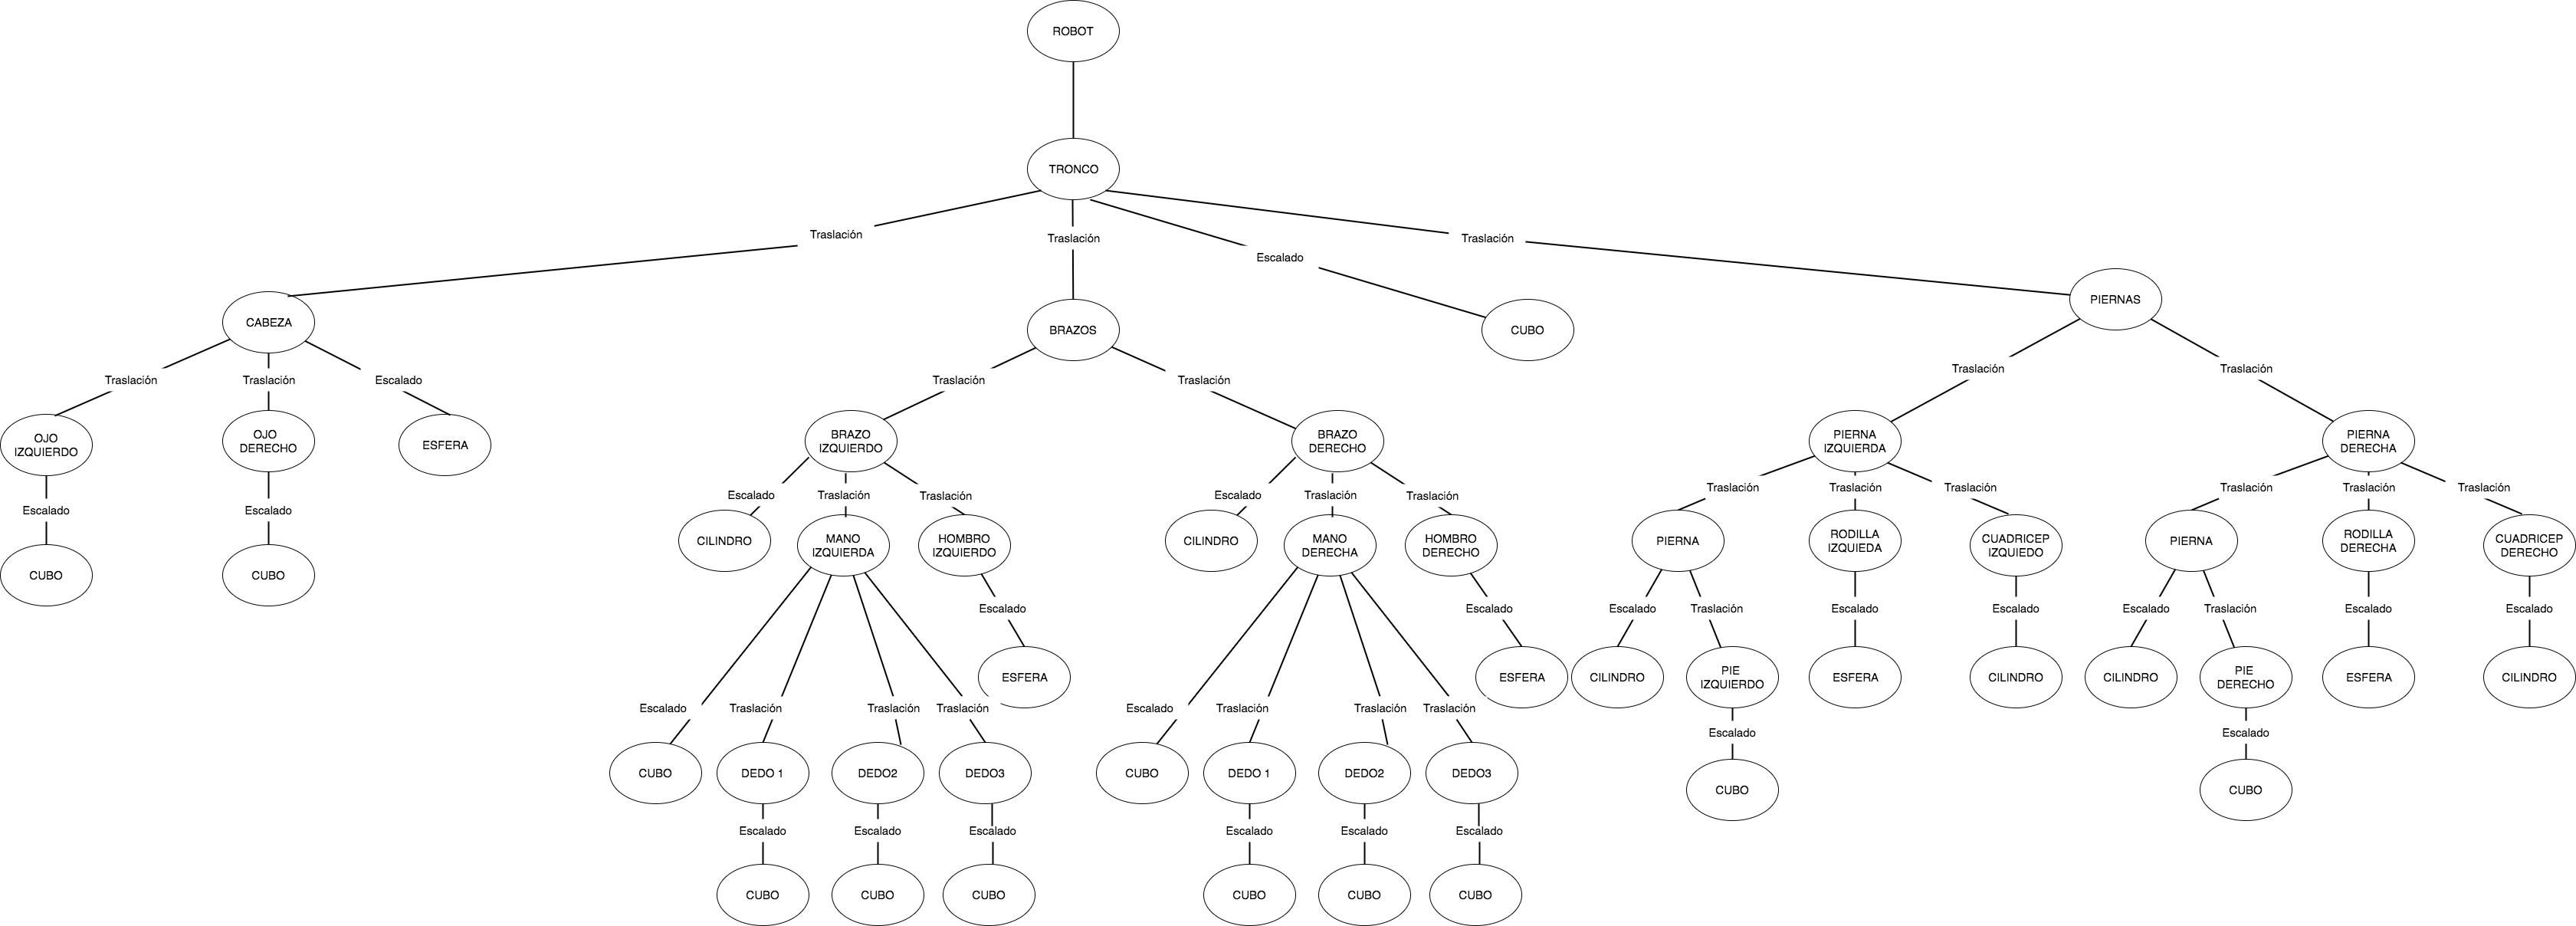
\includegraphics[width = 1.00\textwidth]{Imagenes/p2-img1.png}
 		\captionof{figure}{\label{fig:IPN}Grafo de escena.} 
	\end{center} 
\end{figure}


\section{Desarrollo de la práctica.}

Observando el grafo de escena que se muestra en la imagen anterior, podemos ver que van a ser necesarios un conjunto de objetos primitivos a los cuales se les aplicarán las pertinentes transformaciones indicadas en el grafo para formar el objeto final''Robot''. \\

\subsection{Modelado y transformaciones.}

Como se indica en el grafo, tomaremos un cubo para formar el tronco del objeto, al cual le serán aplicadas transforaciones de escalado y traslación obteniendo el resultado que se ve en la siguiente figura.\\

\begin{figure}[H]
	\begin{center}
	 		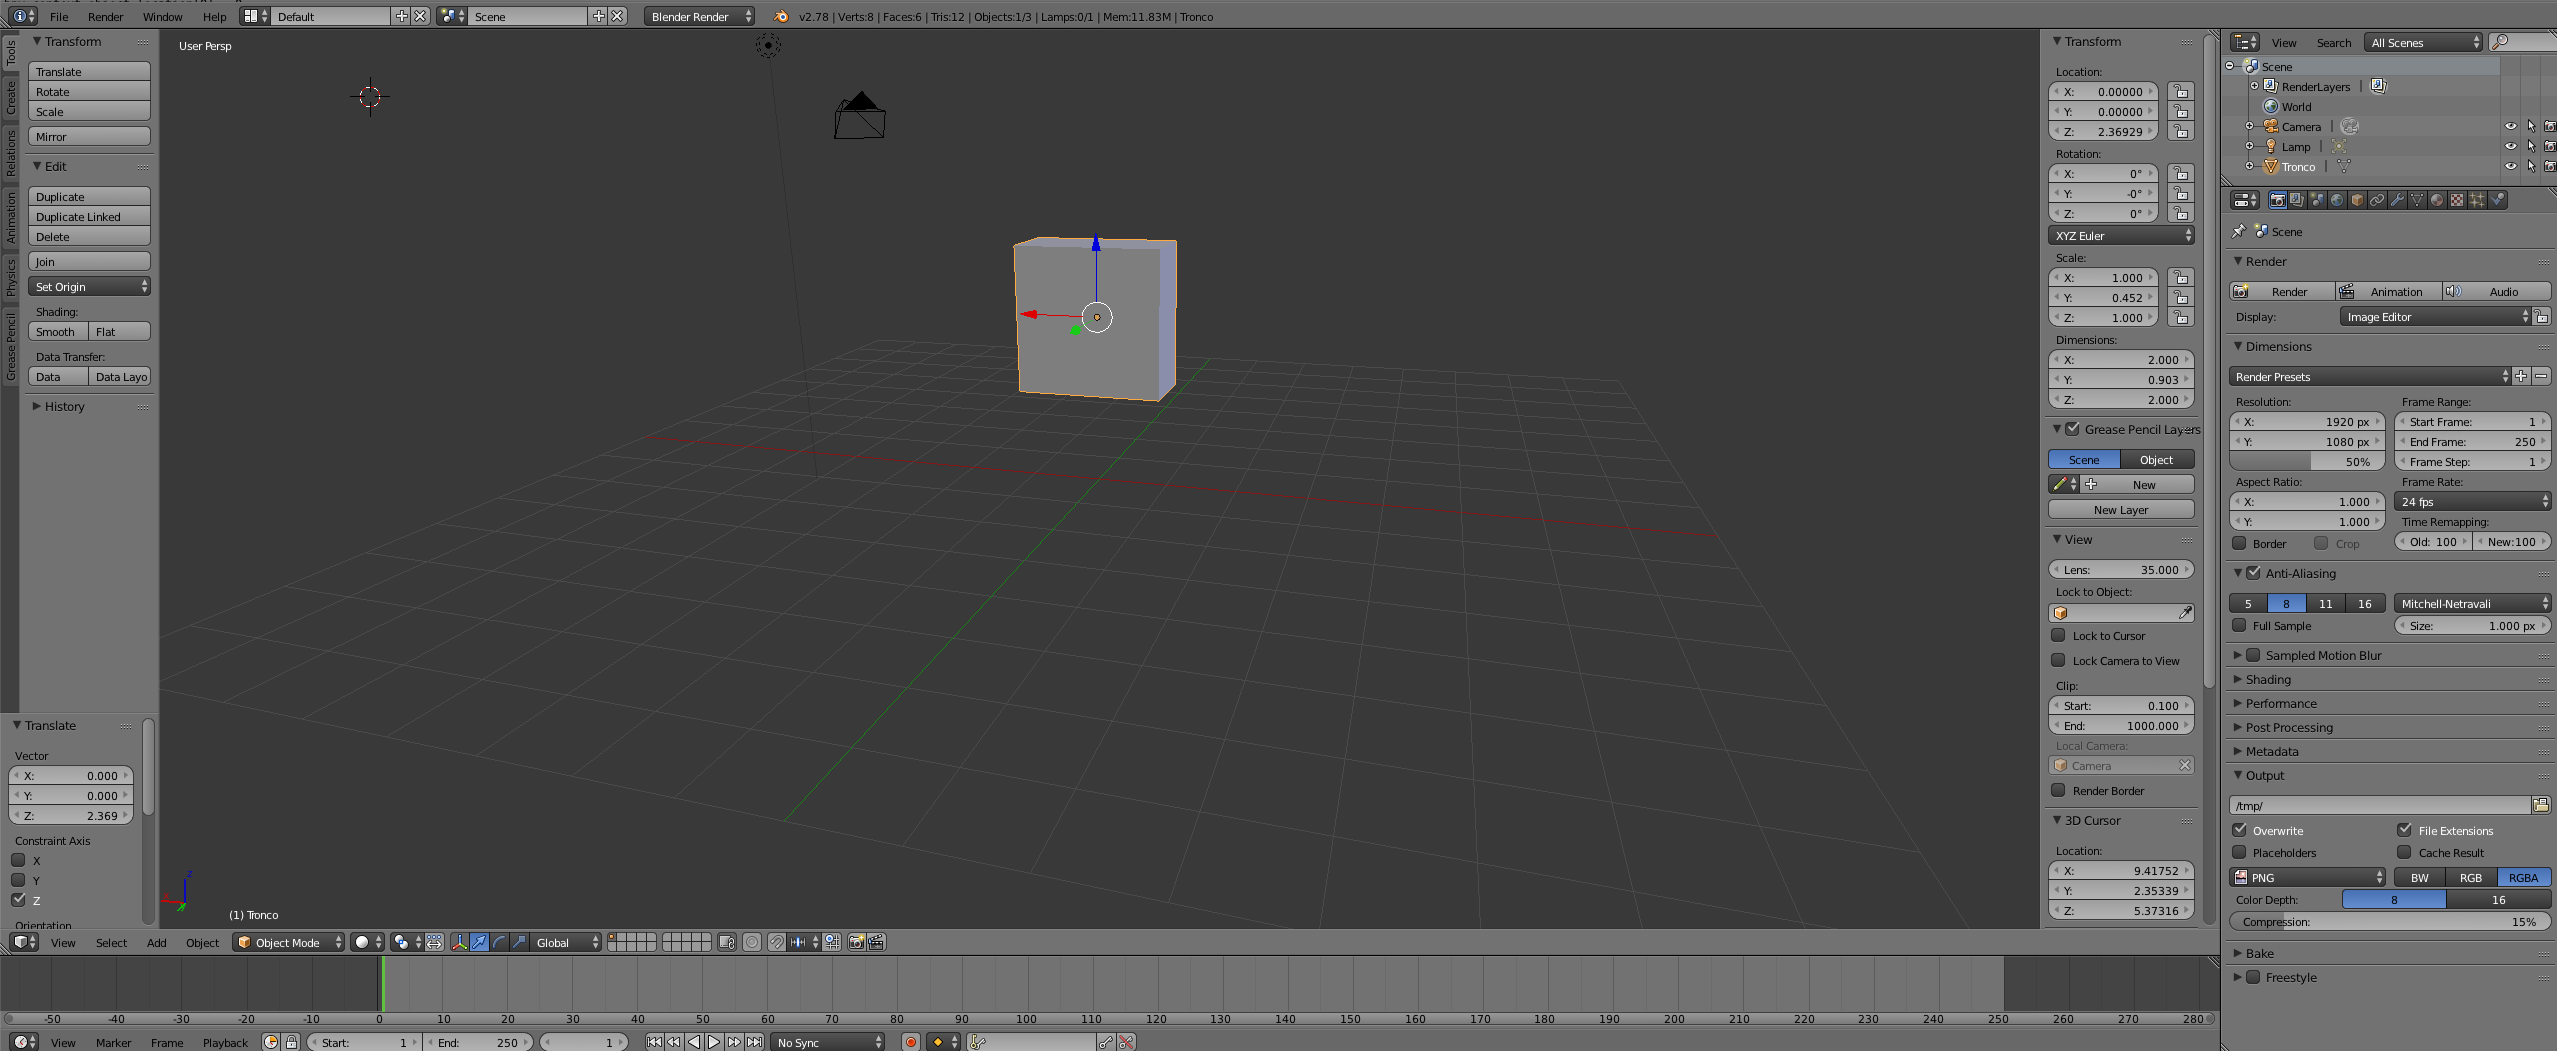
\includegraphics[width = 1.00\textwidth]{Imagenes/p2-img2.png}
 		\captionof{figure}{\label{fig:IPN}Modelado tronco.} 
	\end{center} 
\end{figure}

La siguiente parte del objeto a modelar es la cabeza. Para esta parte será neceario una esfera para la misma y un cubo para cada uno de los ojos. Una vez tengamos dichas figuras le aplicaremos transformaciones de escalado y traslación para conseguir el objeto final ''Cabeza'' como se muestra en la imagen.\\

\begin{figure}[H]
	\begin{center}
	 		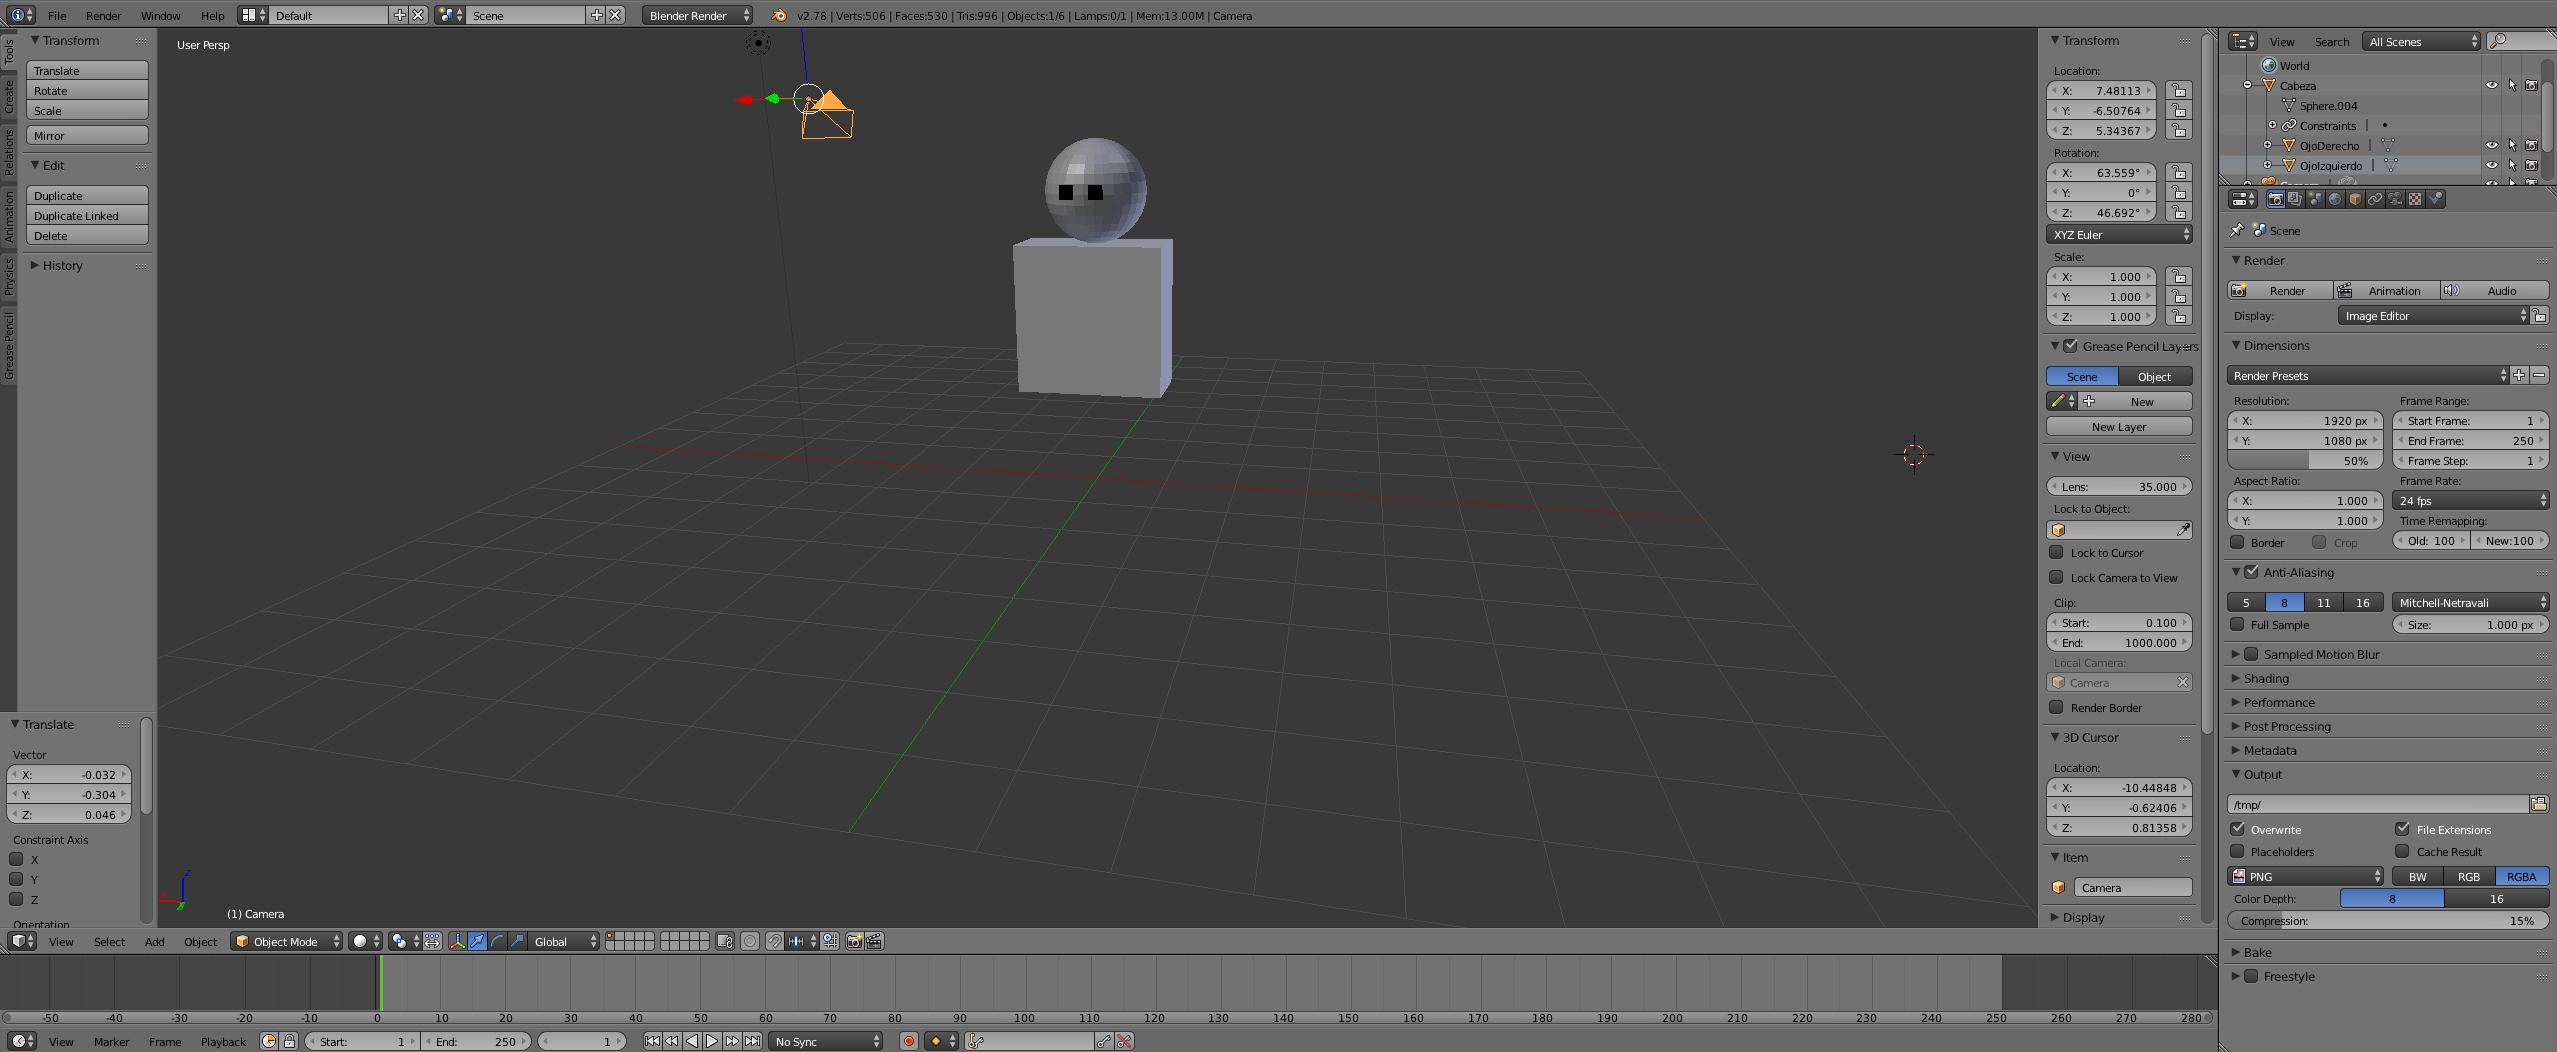
\includegraphics[width = 1.00\textwidth]{Imagenes/p2-img3.png}
 		\captionof{figure}{\label{fig:IPN}Modelado cabeza.} 
	\end{center} 
\end{figure}

Para el modelado del objeto "Brazo", tanto para el izquierdo como para el derecho, han sido necesarios varios tipos de objetos como se puede comprobar en el grafo de escena debido a las partes que lo componen. Ha sido necesaria una esfera para el hombro, un cilindro para el brazo, un cubo para la mano y otros tres para los dedos. Esto mismo se duplica dos veces, una para cada brazo. A todos los objetos se le han aplicado sus correspondientes transformaciones de escalado y traslación para obtener el resultado de la siguiente figura.\\

\begin{figure}[H]
	\begin{center}
	 		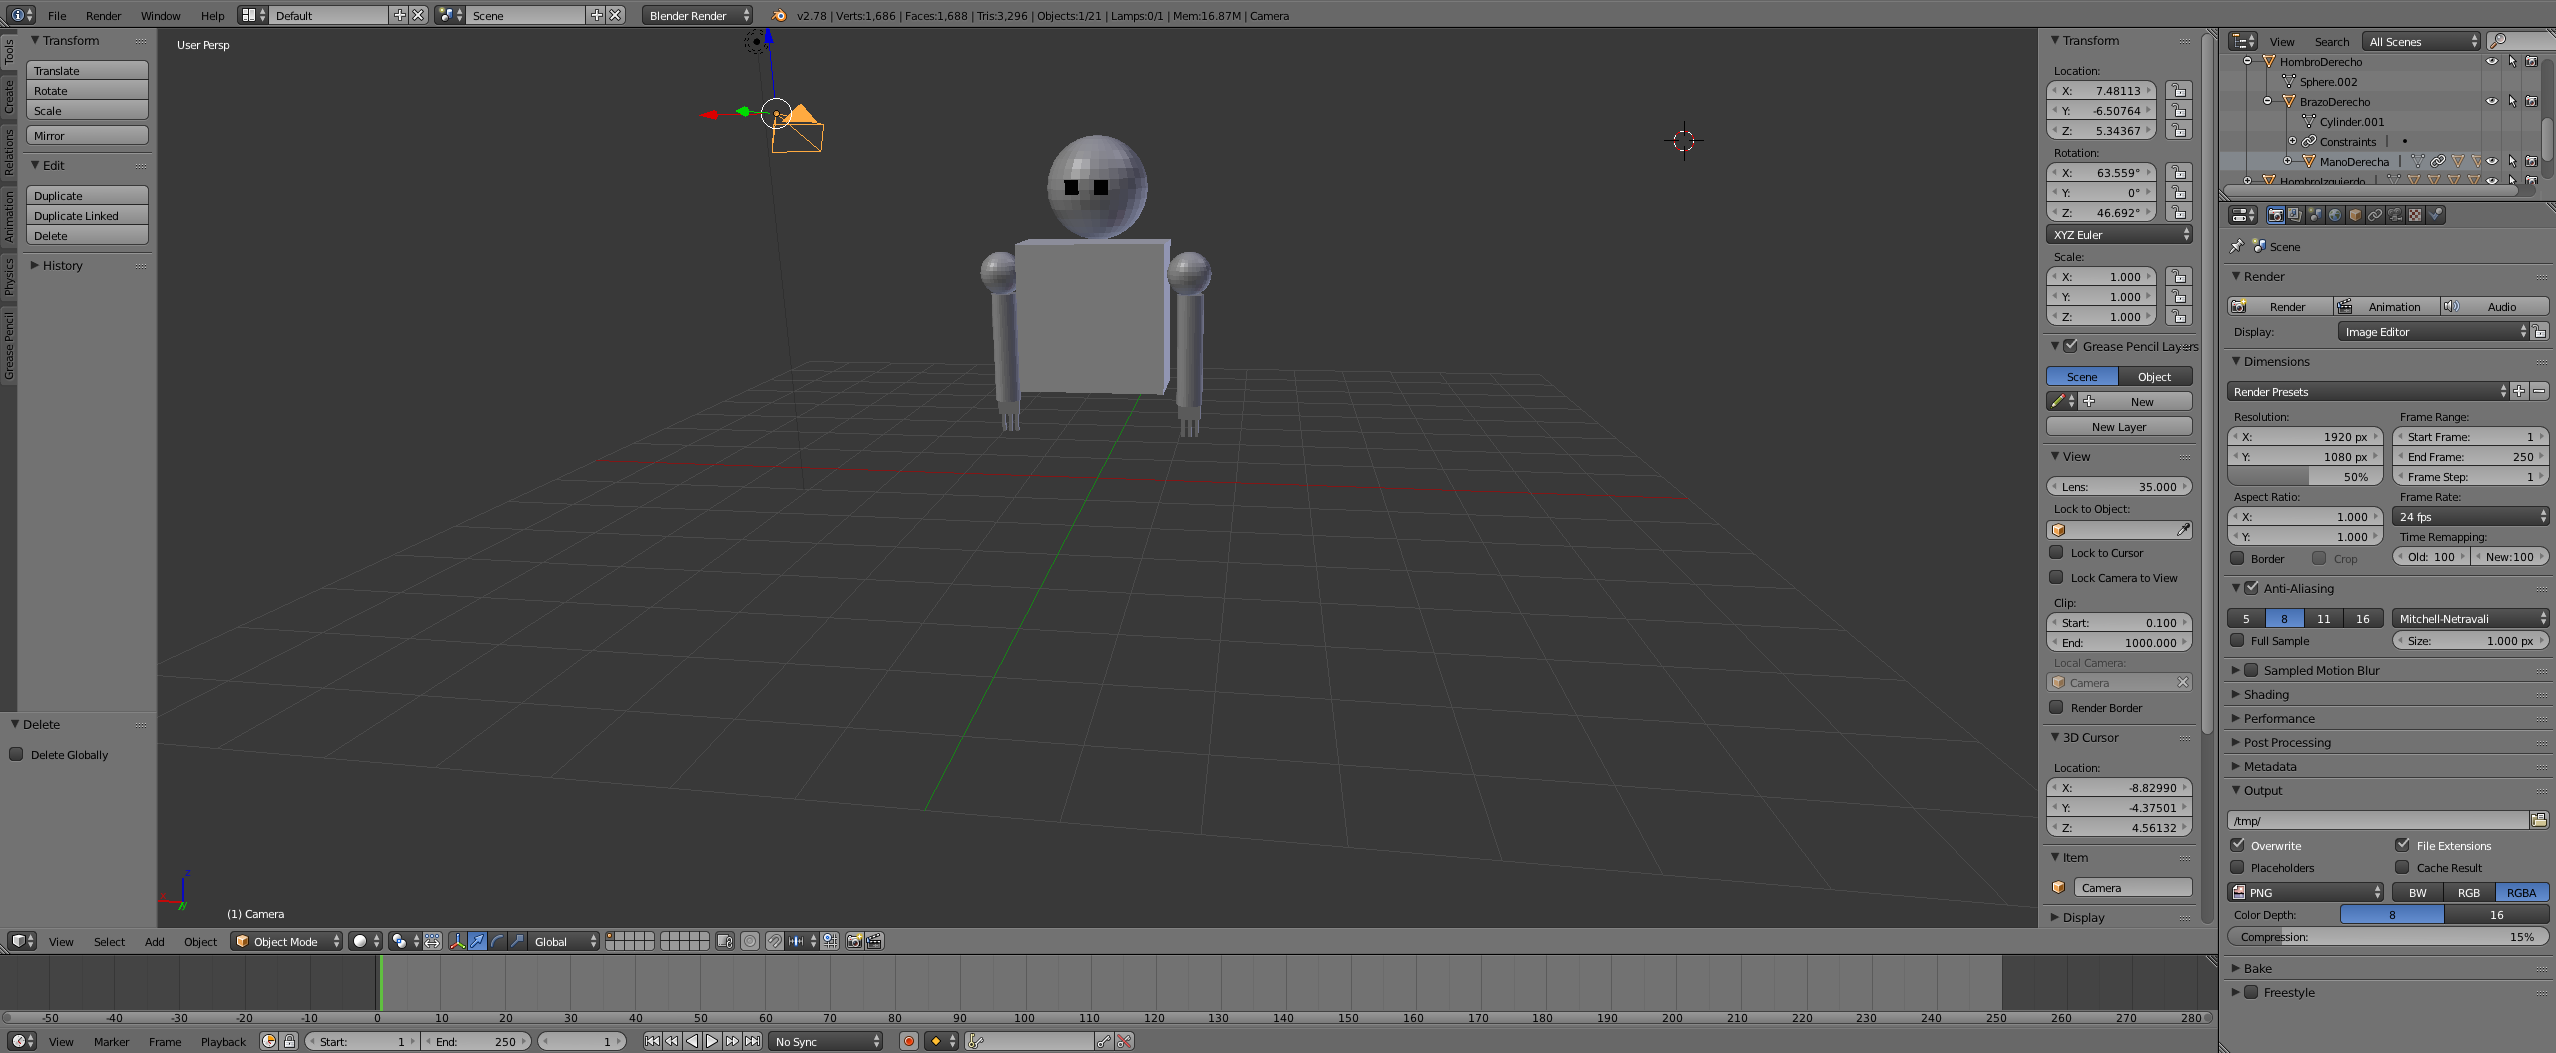
\includegraphics[width = 1.00\textwidth]{Imagenes/p2-img4.png}
 		\captionof{figure}{\label{fig:IPN}Modelado brazo.} 
	\end{center} 
\end{figure}

Aplicaremos el mismo proceso para modelar el objeto "Pierna", al igual que con el objeto anterior un objeto para la pierna izquierda y otro para la pierna derecha. Mirando el grafo se comprueba los diversos objetos que lo componen, asi como las diferentes figuras primitivas. Un objeto cilindro es necesario para el cuadriceps, asi como otro mismo objeto para la pierna en sí. Una figura esfera se emplea para la rodilla mientras que un objeto cubo es utilizado para el pie, todos estos objetos se necesitan por duplicado para modelar las dos piernas. A continuación se le aplicarán a dichos objetos las pertinentes transformaciones de escalado y translación como marca el grafo de escena y conseguir el mismo efecto que se puede ver en la siguiente imagen. \\ \\ \\ \\ \\

\begin{figure}[H]
	\begin{center}
	 		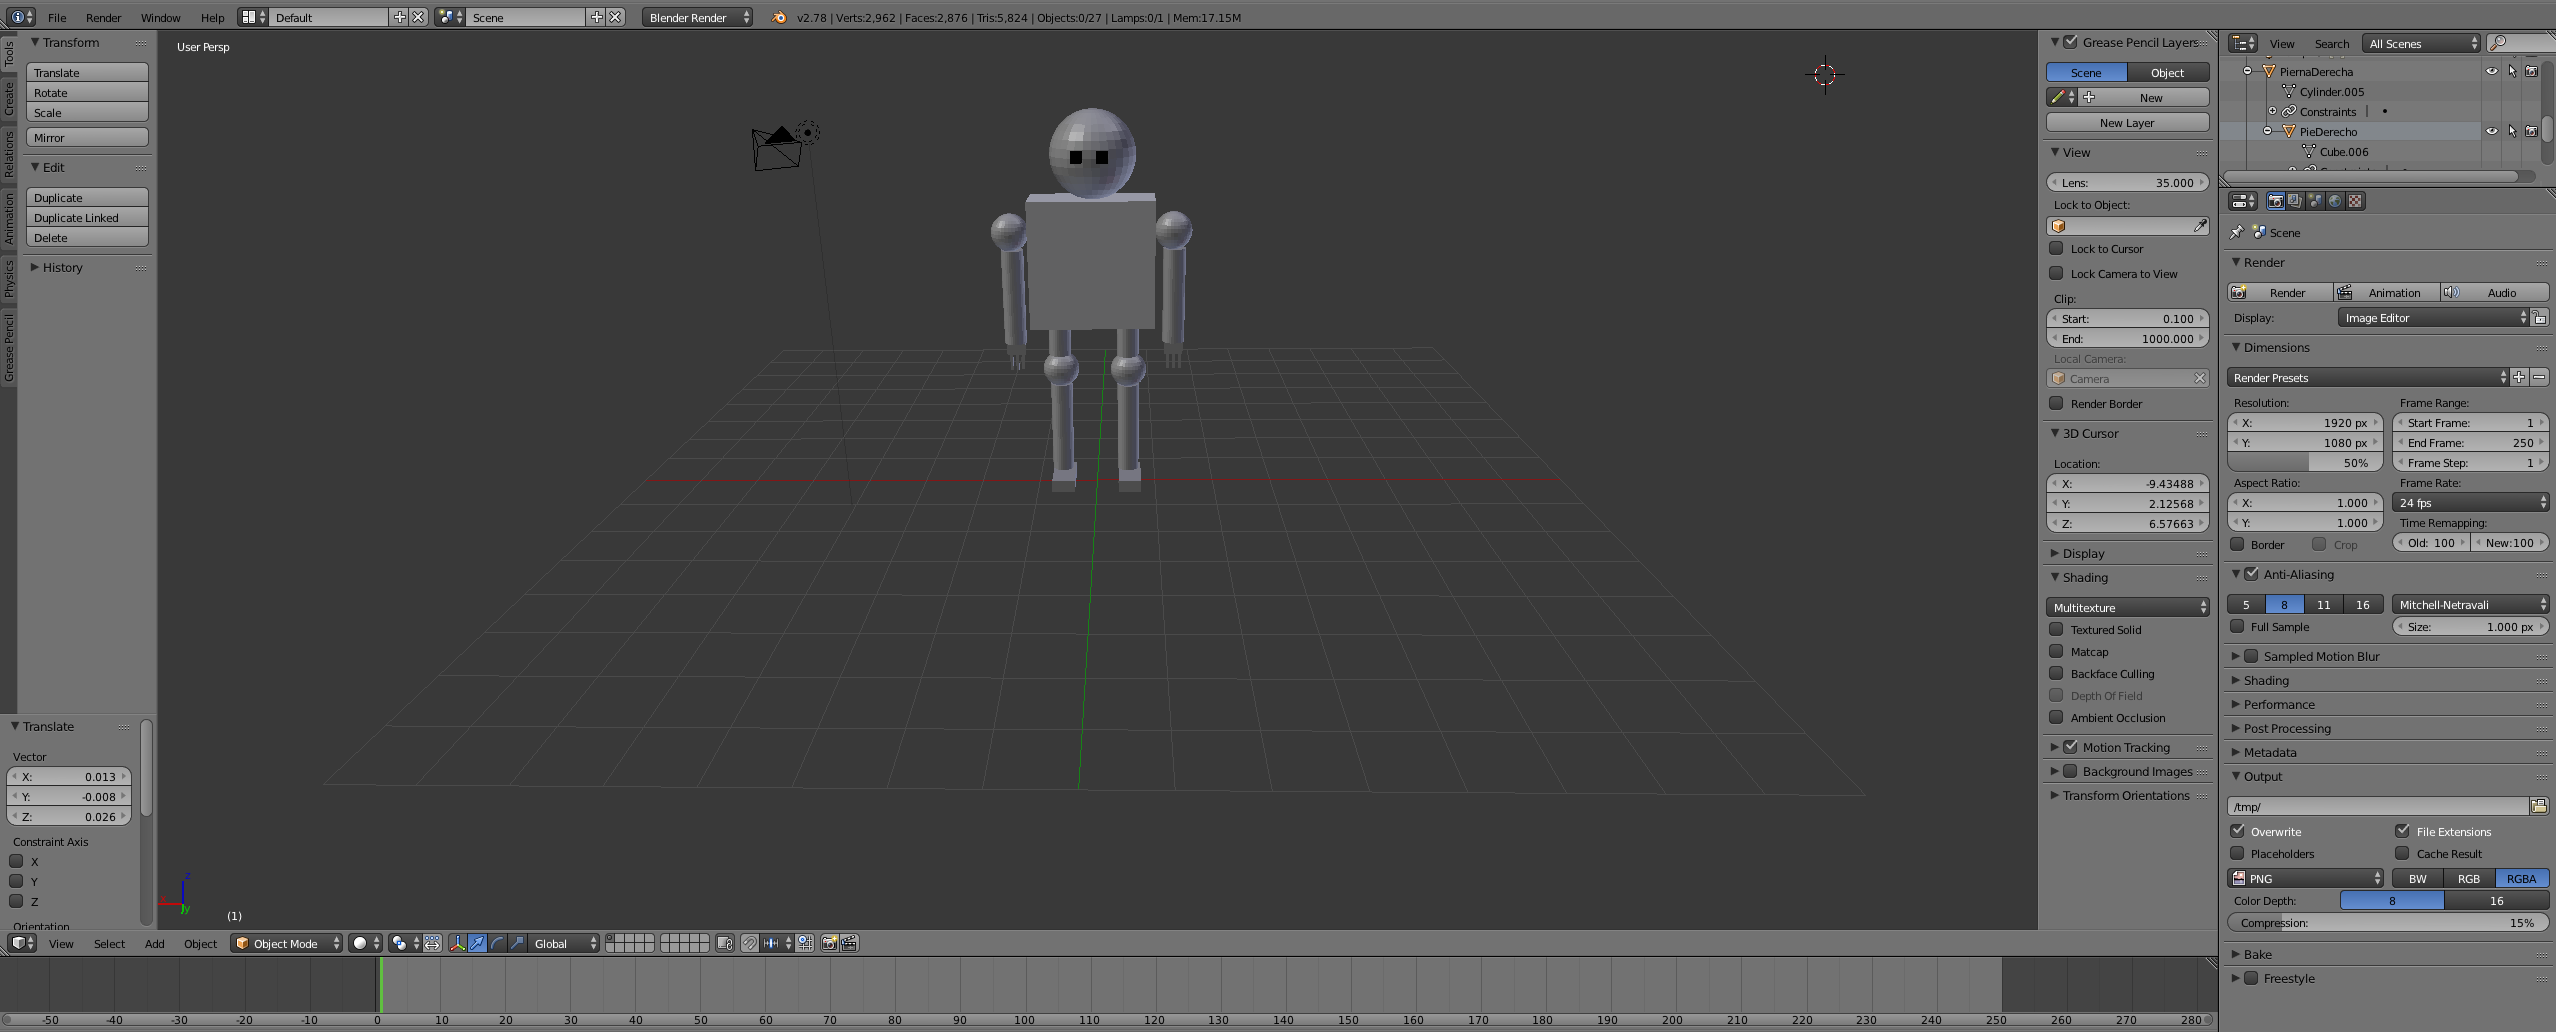
\includegraphics[width = 1.00\textwidth]{Imagenes/p2-img5.png}
 		\captionof{figure}{\label{fig:IPN}Modelado pierna.} 
	\end{center} 
\end{figure}

El resultado final del objeto después de haber realizado todas las transformaciones es el que se muestra en la siguiente figura.\\

\begin{figure}[H]
	\begin{center}
	 		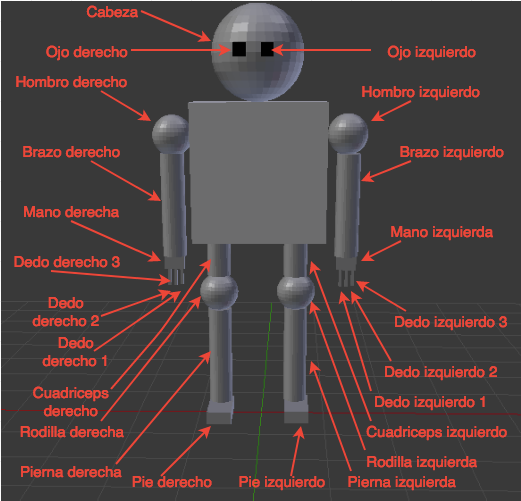
\includegraphics[width = 0.75\textwidth]{Imagenes/p2-img17.png}
 		\captionof{figure}{\label{fig:IPN}Figura Robot.} 
	\end{center} 
\end{figure}

\subsection{Restricciones y movimientos.}

Una vez que tenemos modelado el objeto, lo siguiente es asignar los movimientos a las partes que son articuladas asi como restringírlas a las que no lo son. Son varias las partes del objeto que tienen movilidad, para la cual se ha tenido que realizar una serie de procedimientos que se detallarán en este apartado. \\

Comenzando con el objeto ''Cabeza'', el cilindro empleado para ello tiene restringidas las rotaciones tanto en el eje X como en el Y, siendo solamente posible realizar en el eje Z la rotación. A esta transformación en dicho eje se le ha establecido una limitación de -90º como valor mínimo y de 90º como máximo. Los dos cubos que representan a cada uno de los ojos tienen restringidas las rotaciones en los tres ejes (X, Y, Z). En las figuras 7 y 8 se puede ver el resultado.\\

\begin{figure}[H]
	\begin{center}
	 		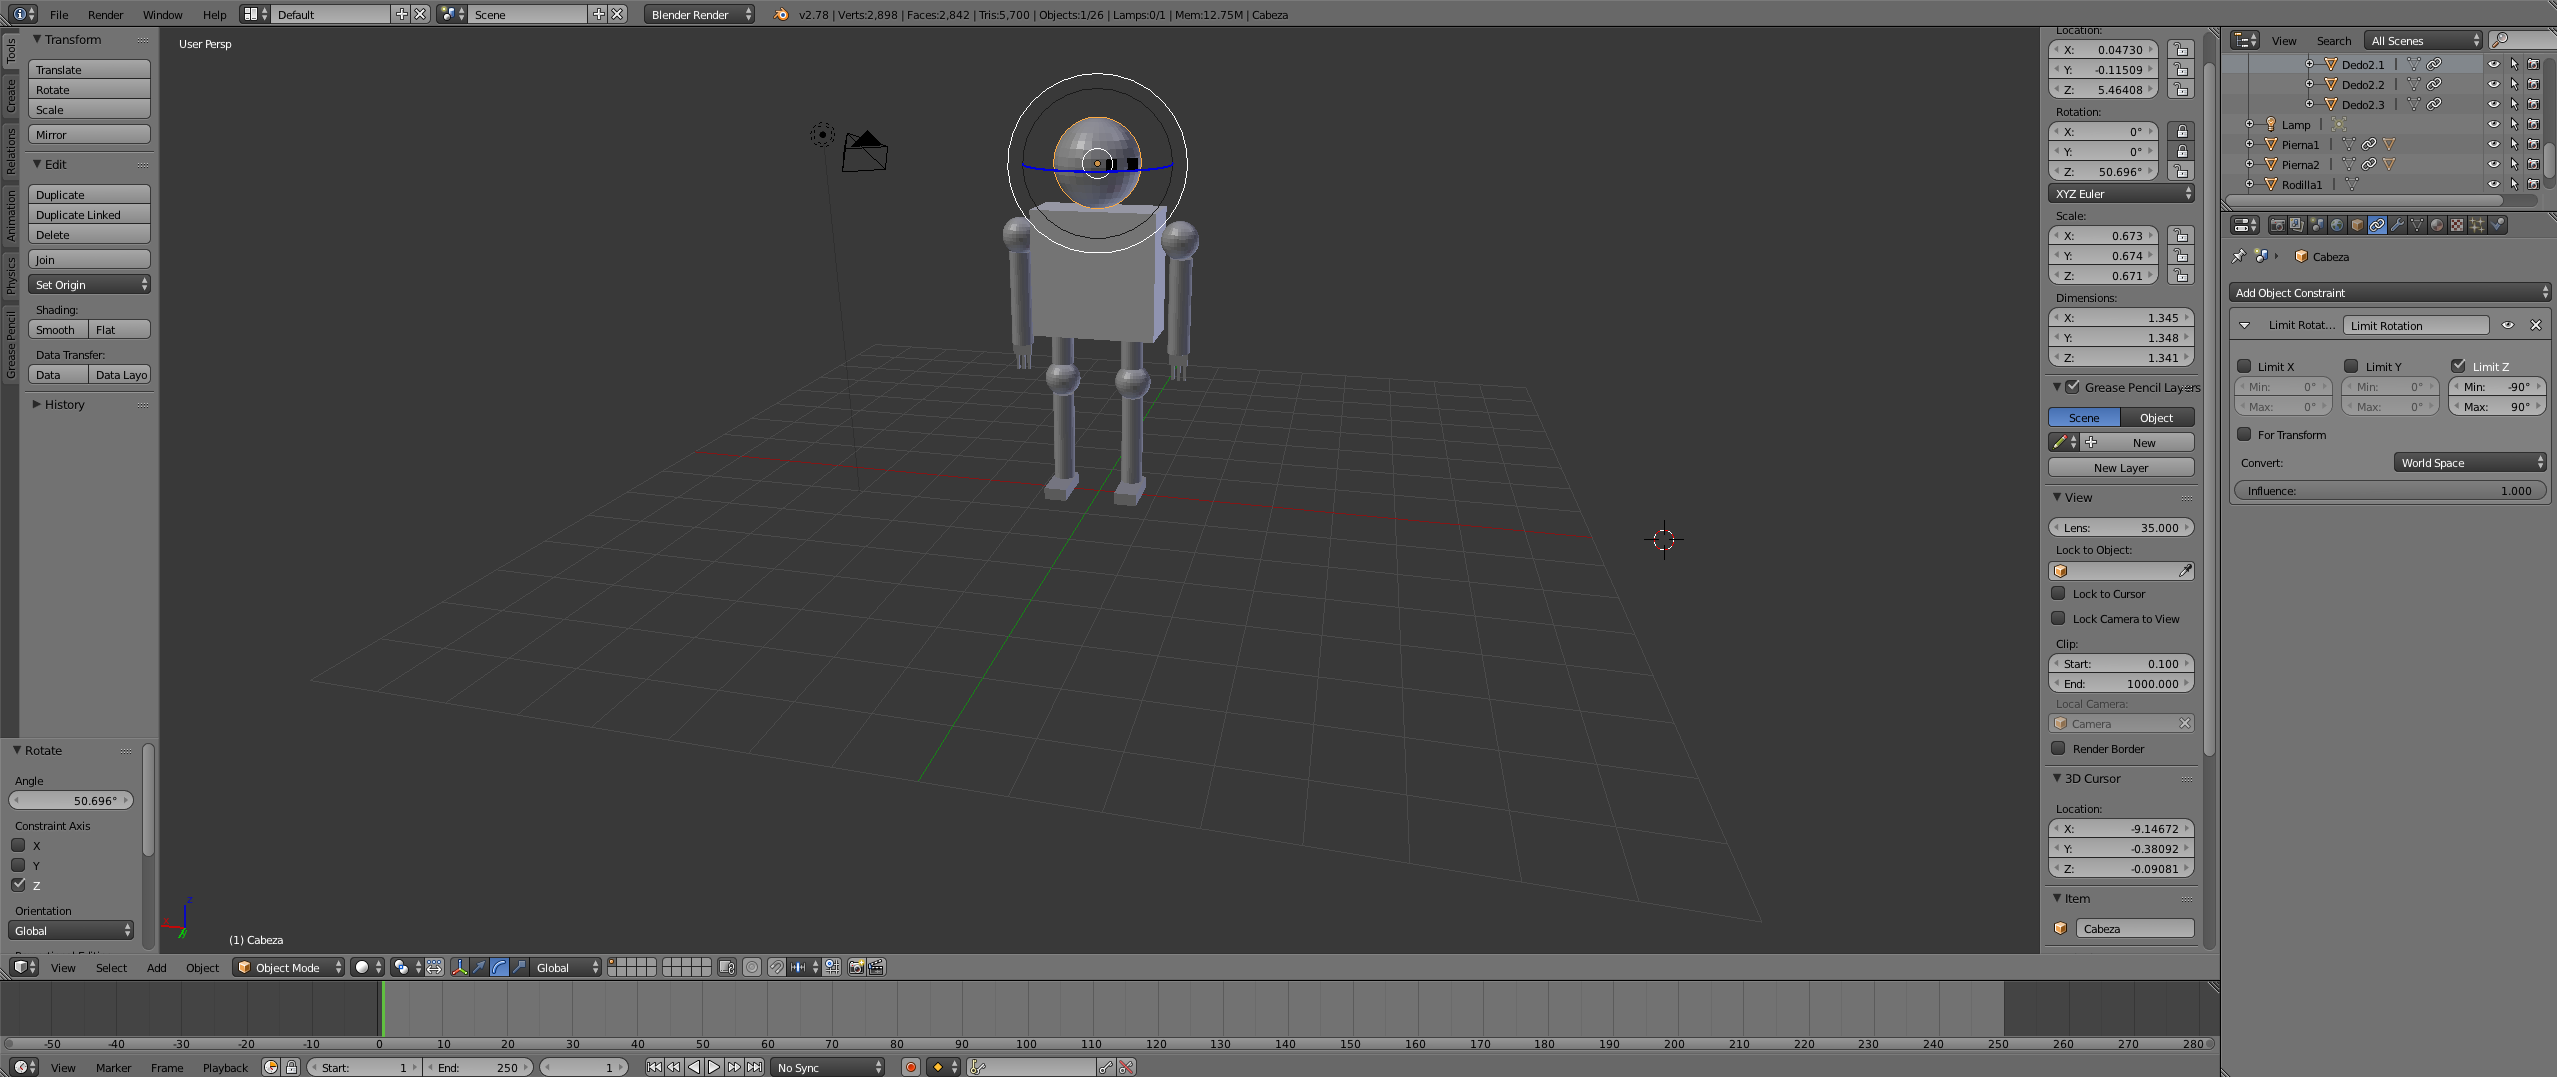
\includegraphics[width = 1.00\textwidth]{Imagenes/p2-img6.png}
 		\captionof{figure}{\label{fig:IPN}Rotación en la cabeza (I).} 
	\end{center} 
\end{figure}

\begin{figure}[H]
	\begin{center}
	 		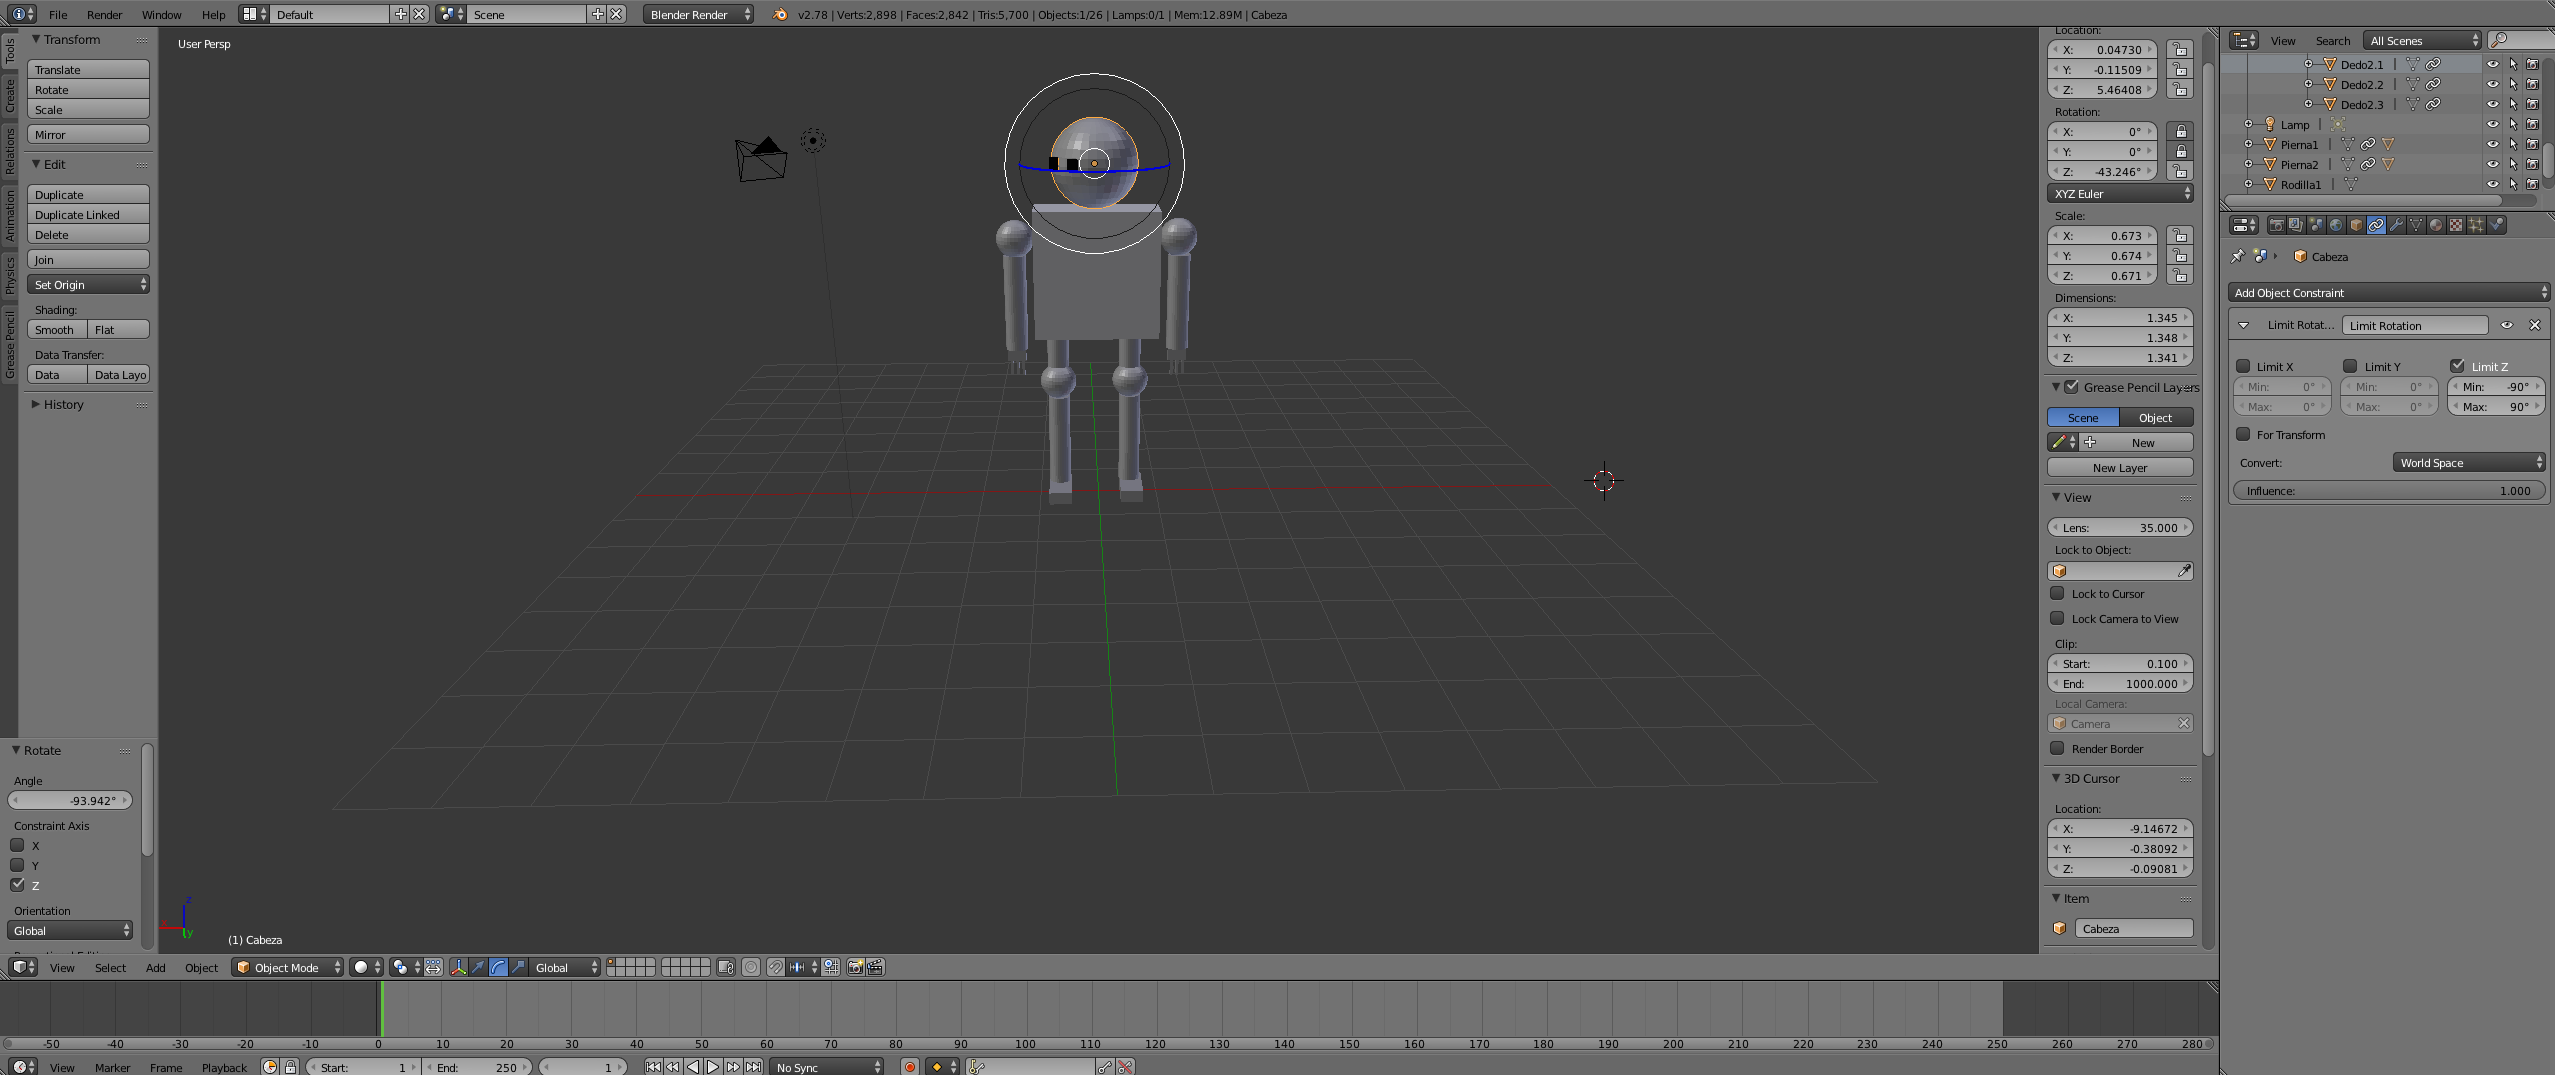
\includegraphics[width = 1.00\textwidth]{Imagenes/p2-img7.png}
 		\captionof{figure}{\label{fig:IPN}Rotación en la cabeza (II).} 
	\end{center} 
\end{figure}

Siguiendo con las partes que forman el objeto''Robot'', hemos podido ver en el grafo como el objeto "Brazo" se compone de varios elementos teniendo cada uno de ellos su respectiva figura que lo representa. Para el objeto hombro se ha empleado una esfera a la cual se le han restringido las rotaciones en los tres ejes, siendo por tanto un objeto no articulado. Un cilindro es la figura utilizada para el brazo en sí, al cual se le permiten rotaciones solamente en el eje Z con un valor mínimo de 0º y un máximo de 90º en lo que a la limitación se refiere. Ha sido también necesario modificar su punto de origen para que la rotación fuera la correcta, colocándolo en el punto mas bajo de la esfera que representa el hombro. La mano se representa mediante un cubo que permite rotación limitada con valor mínimo de 0º y máximo de 45º en el eje X y de 0º y 90º en el eje Z como valores mínimo y máximo respectivamente, teniendo restringida las rotaciones en el eje Y. Para este objeto también ha sido necesario modificar el punto de origen, colocandolo en el centro de la cara inferior del cilindro que representa a la mano. \\ \\ \\

Por último, para los objetos de los dedos se han empleado nuevamente figuras de cubo, en este caso para los tres dedos que compone cada mano. Para cada uno de estos objetos se han restringido las transformaciones de rotación en los ejes Y y Z, permitiendo únicamente dicha transformación en el eje X con unos valores mínimo y máximo de -45º y 45º respectivamente de limitación. En estos tres objetos ha sido necesario también modificar el punto de origen para colocarlo en la cara inferior del cubo que representa a la mano. Cabe recordar que esto se realiza para cada uno de los dos brazos que tiene el objeto ''Robot''.\\

\begin{figure}[H]
	\begin{center}
	 		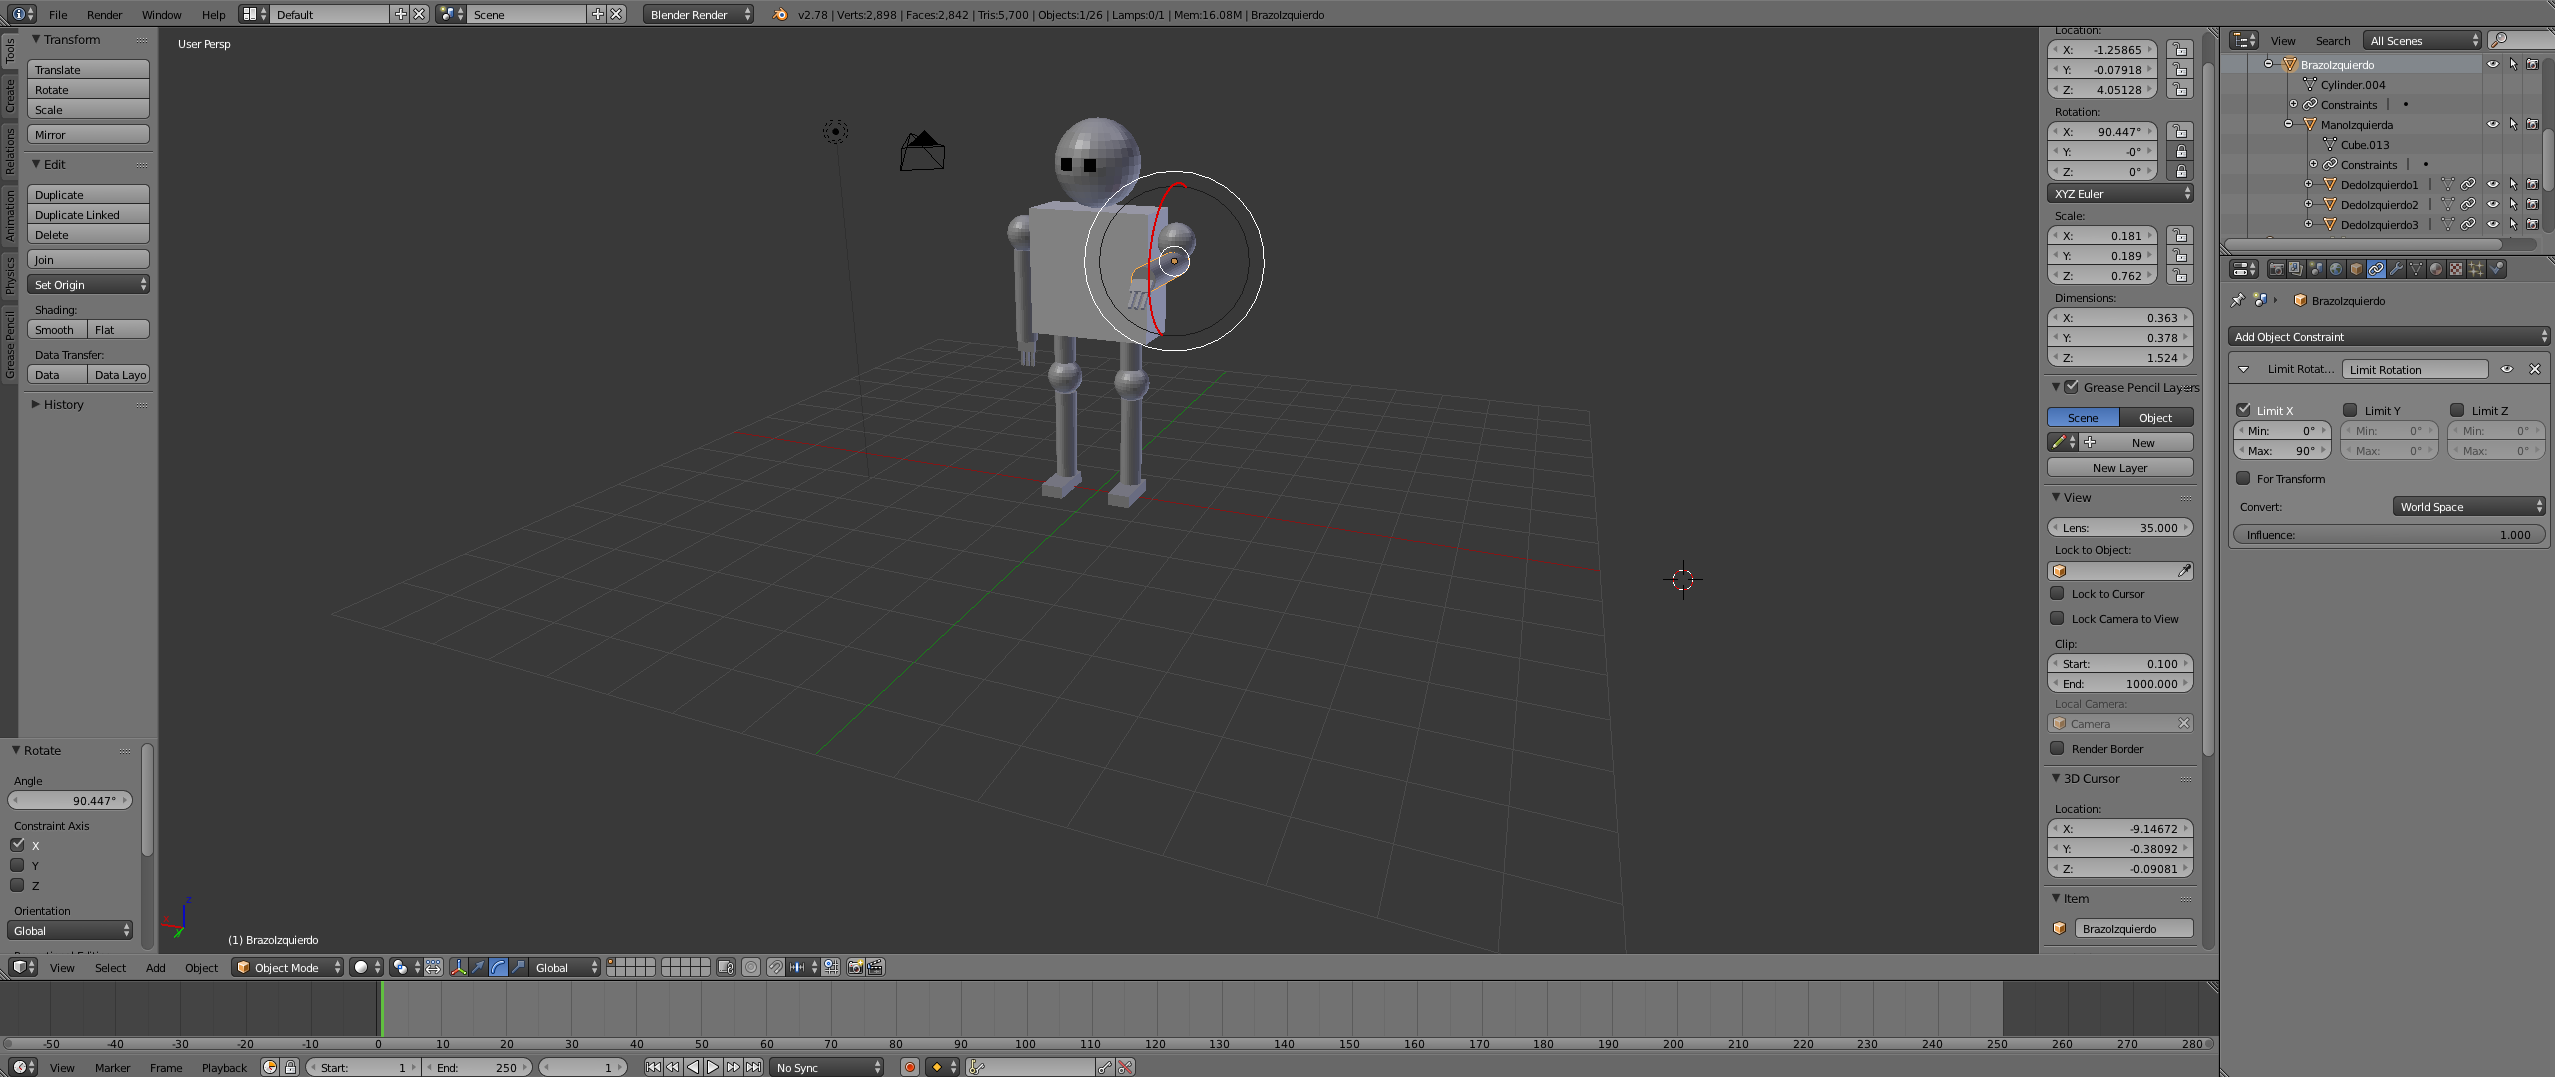
\includegraphics[width = 1.00\textwidth]{Imagenes/p2-img8.png}
 		\captionof{figure}{\label{fig:IPN}Rotación en el brazo (I).} 
	\end{center} 
\end{figure}

\begin{figure}[H]
	\begin{center}
	 		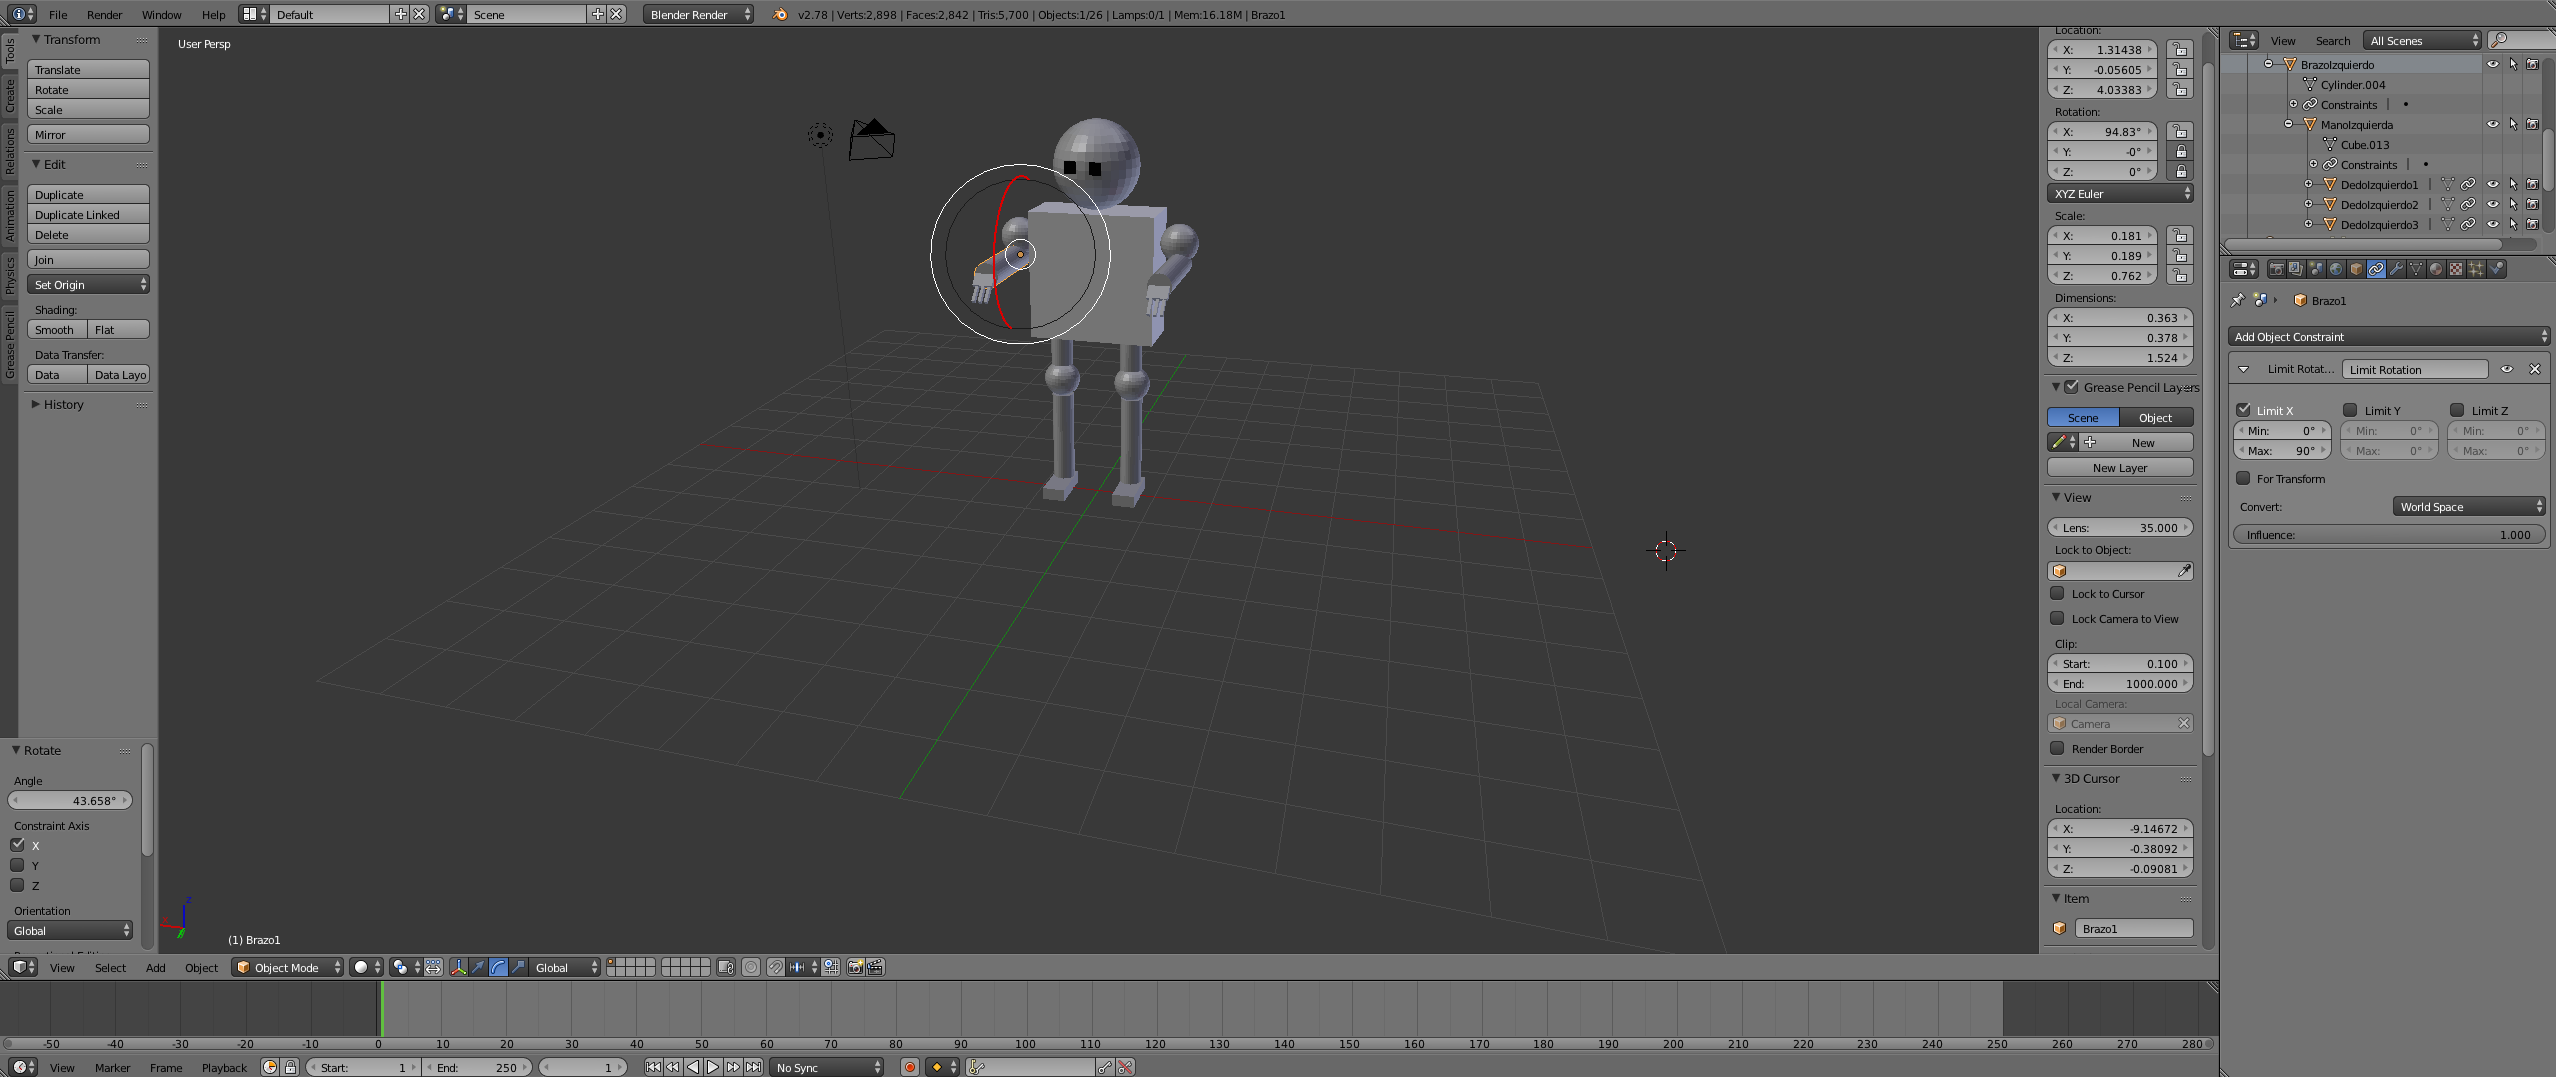
\includegraphics[width = 1.00\textwidth]{Imagenes/p2-img9.png}
 		\captionof{figure}{\label{fig:IPN}Rotación en el brazo (II).} 
	\end{center} 
\end{figure}

\begin{figure}[H]
	\begin{center}
	 		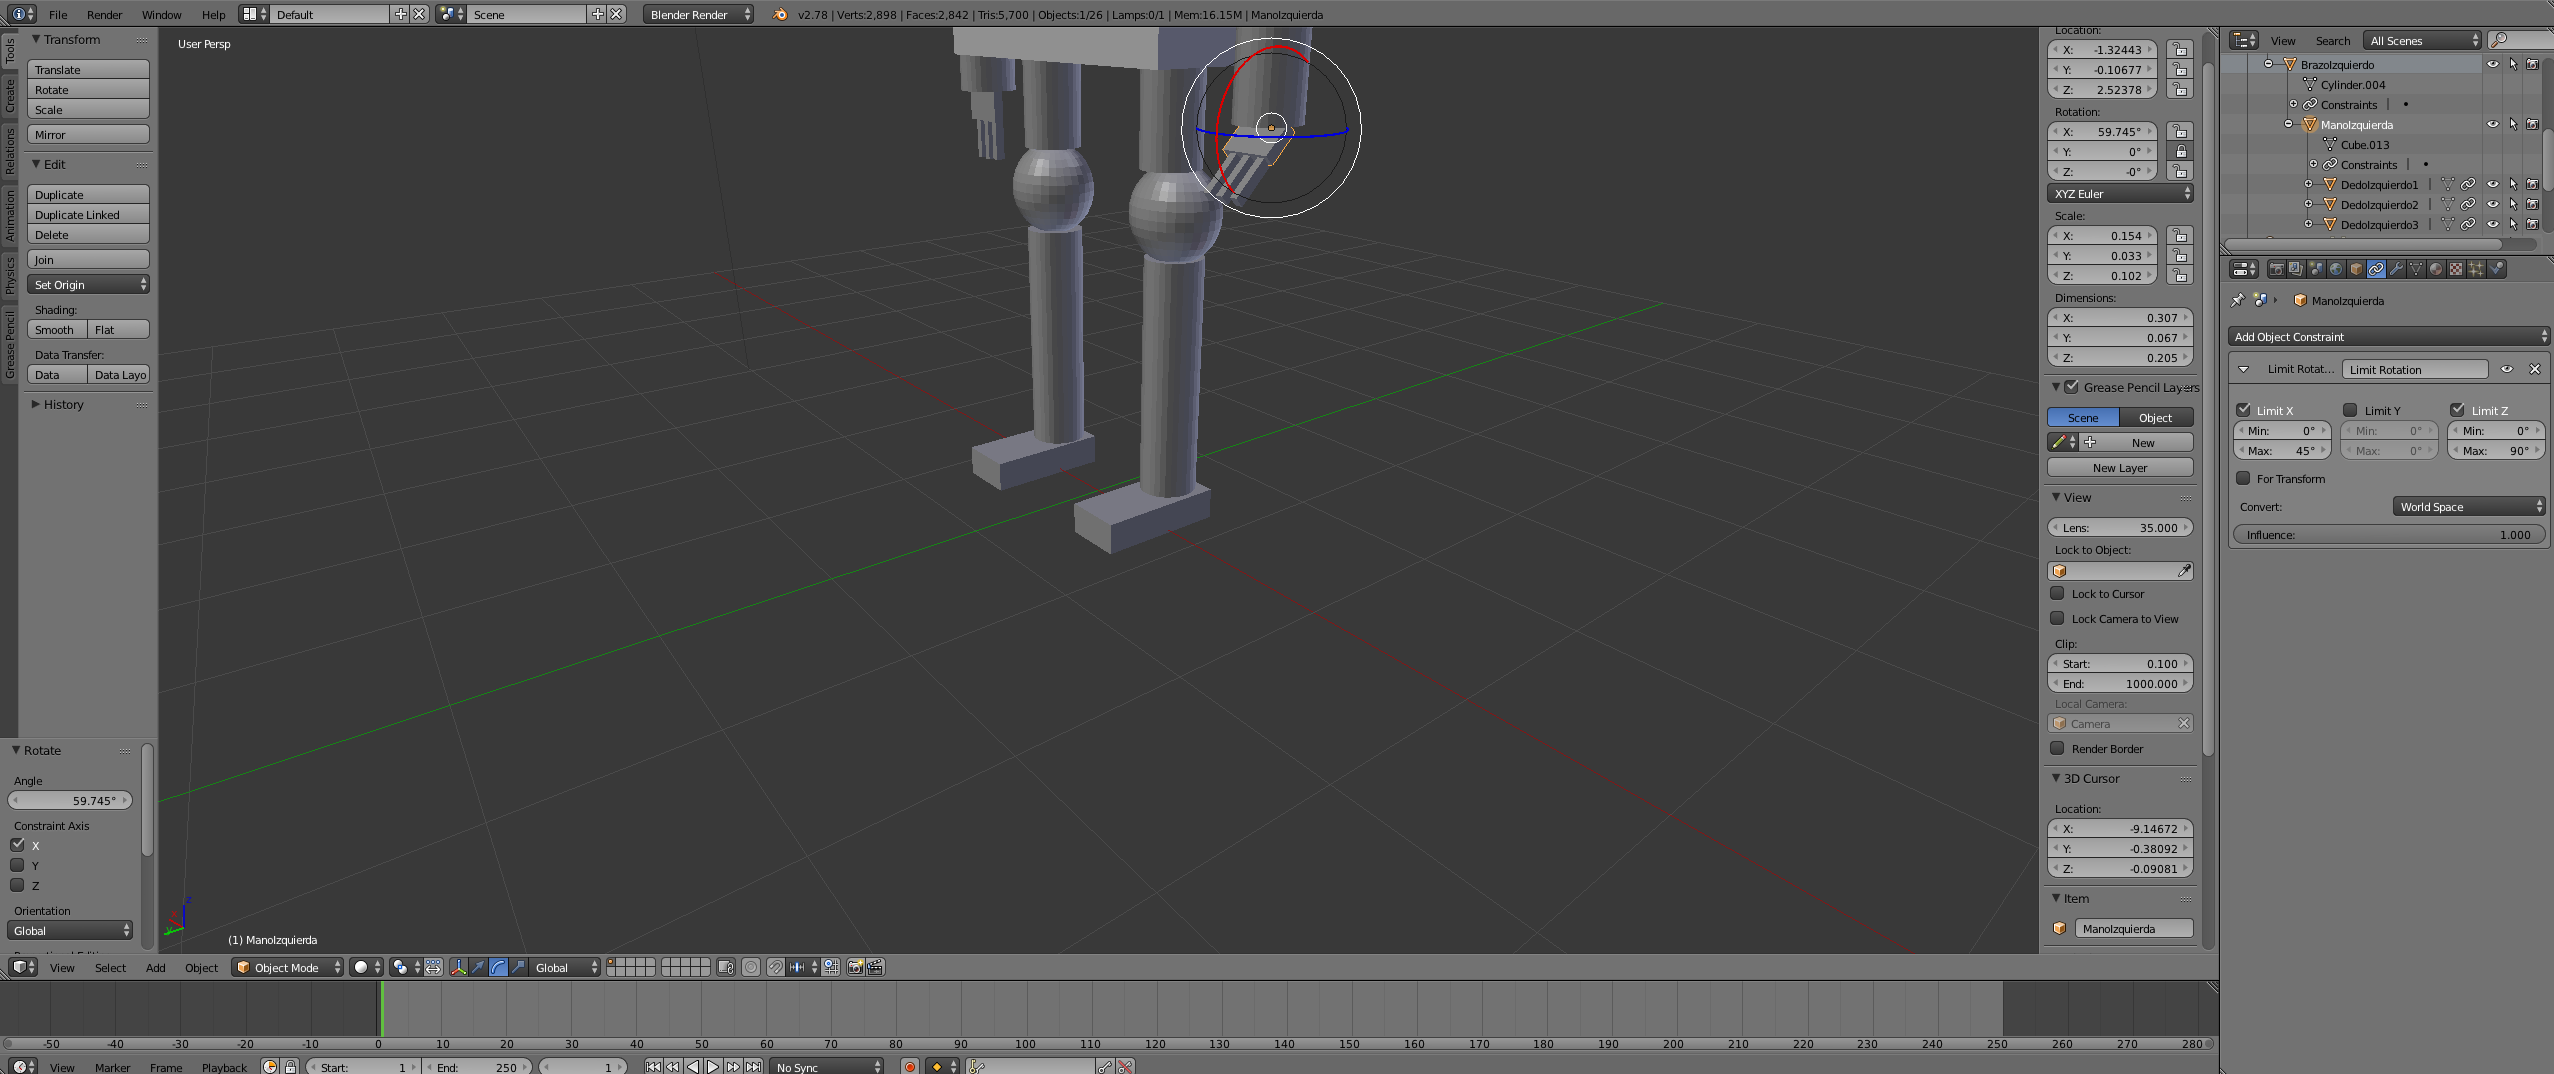
\includegraphics[width = 1.00\textwidth]{Imagenes/p2-img10.png}
 		\captionof{figure}{\label{fig:IPN}Rotación en la mano (I).} 
	\end{center} 
\end{figure}

\begin{figure}[H]
	\begin{center}
	 		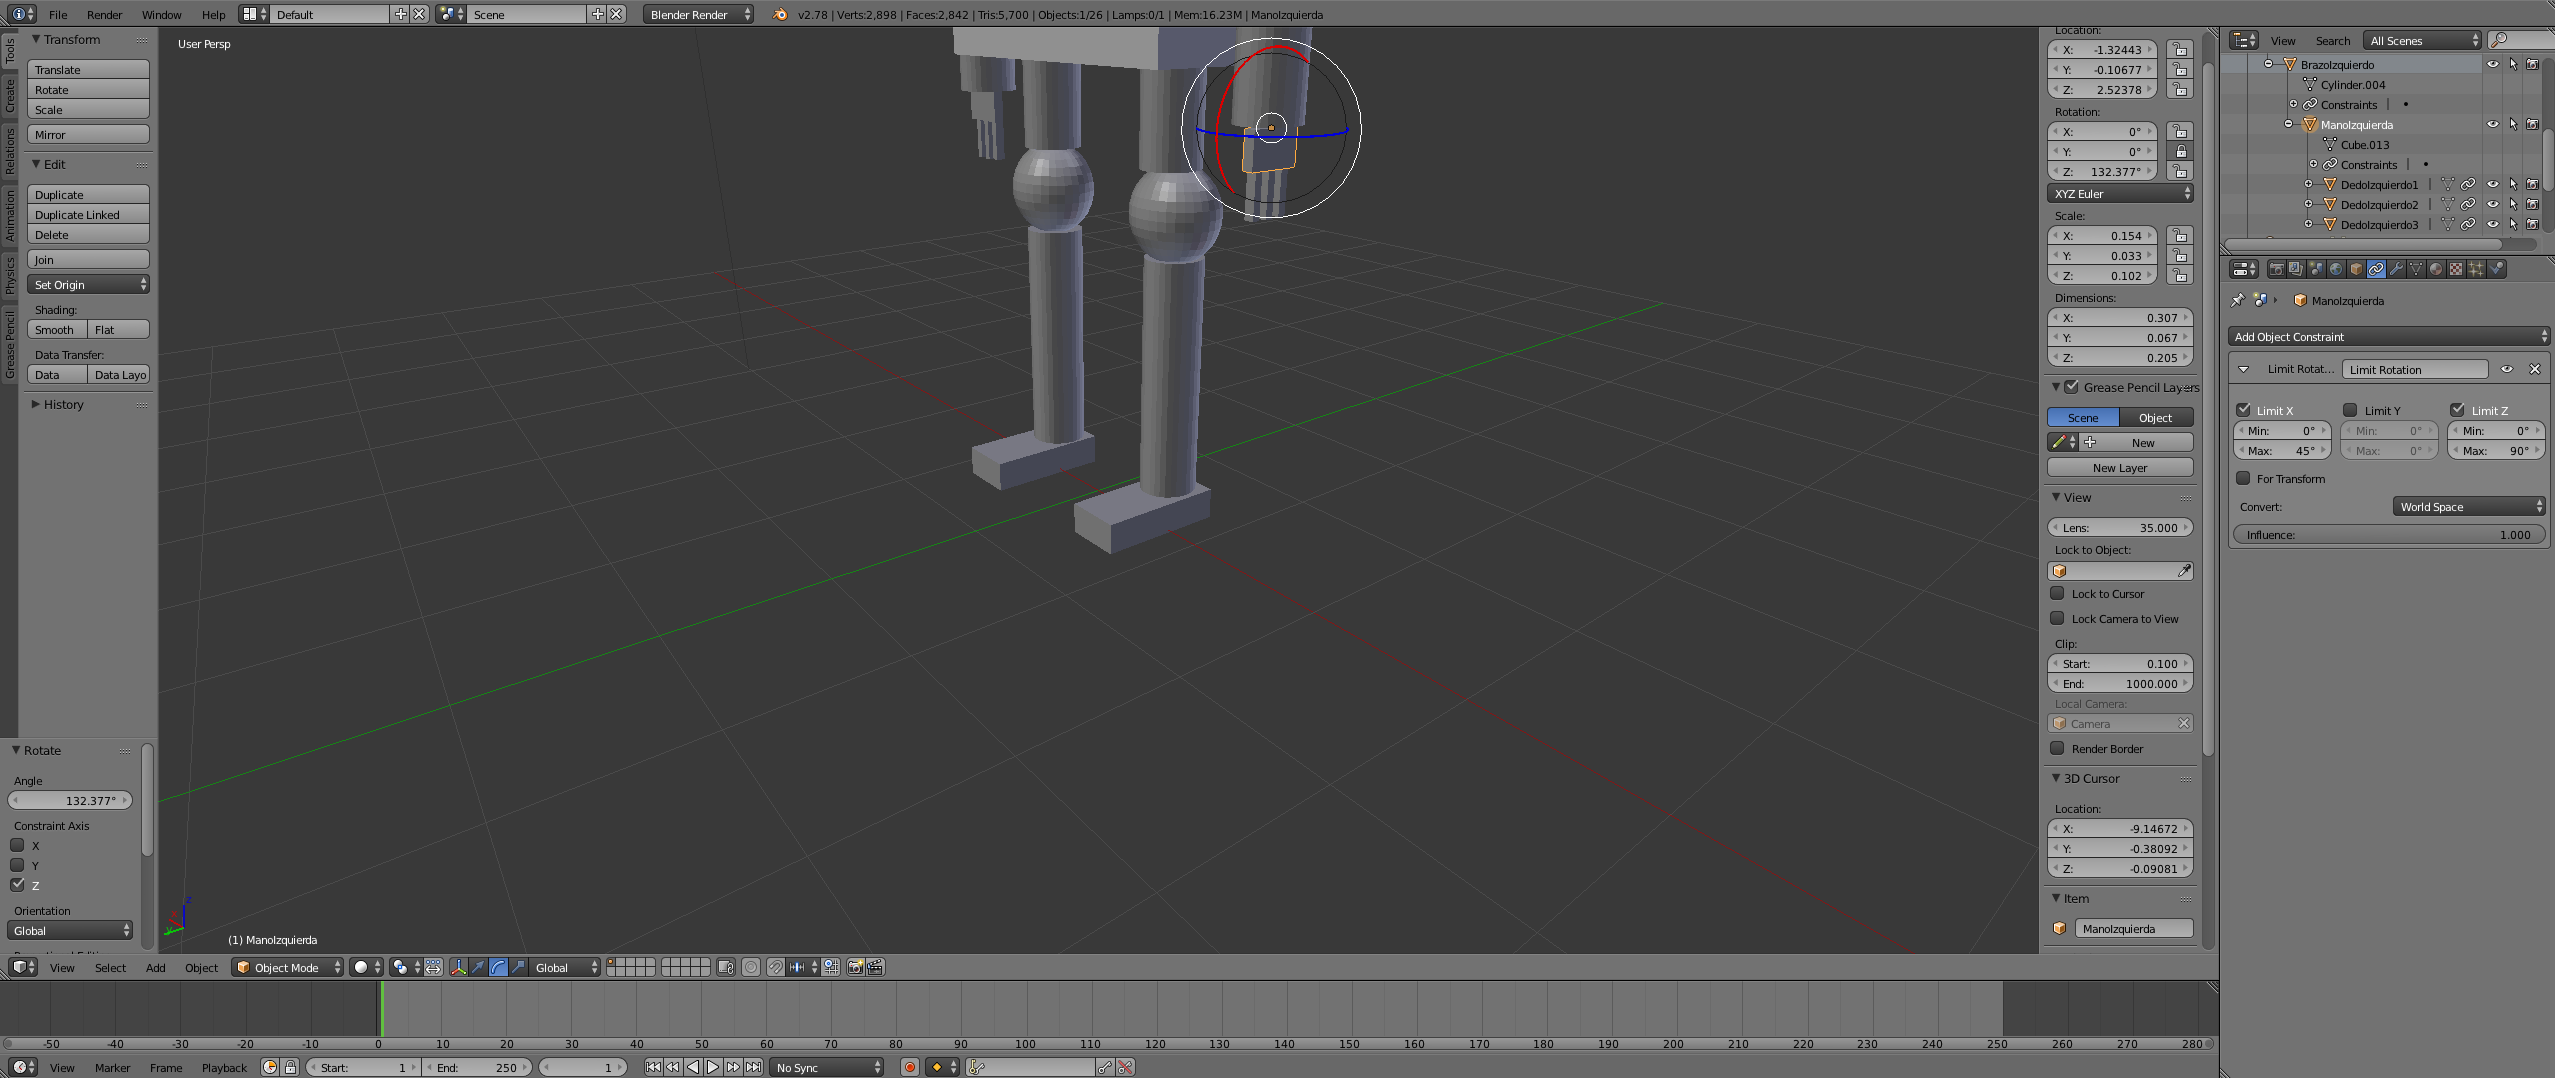
\includegraphics[width = 1.00\textwidth]{Imagenes/p2-img11.png}
 		\captionof{figure}{\label{fig:IPN}Rotación en la mano (!I).} 
	\end{center} 
\end{figure}

\begin{figure}[H]
	\begin{center}
	 		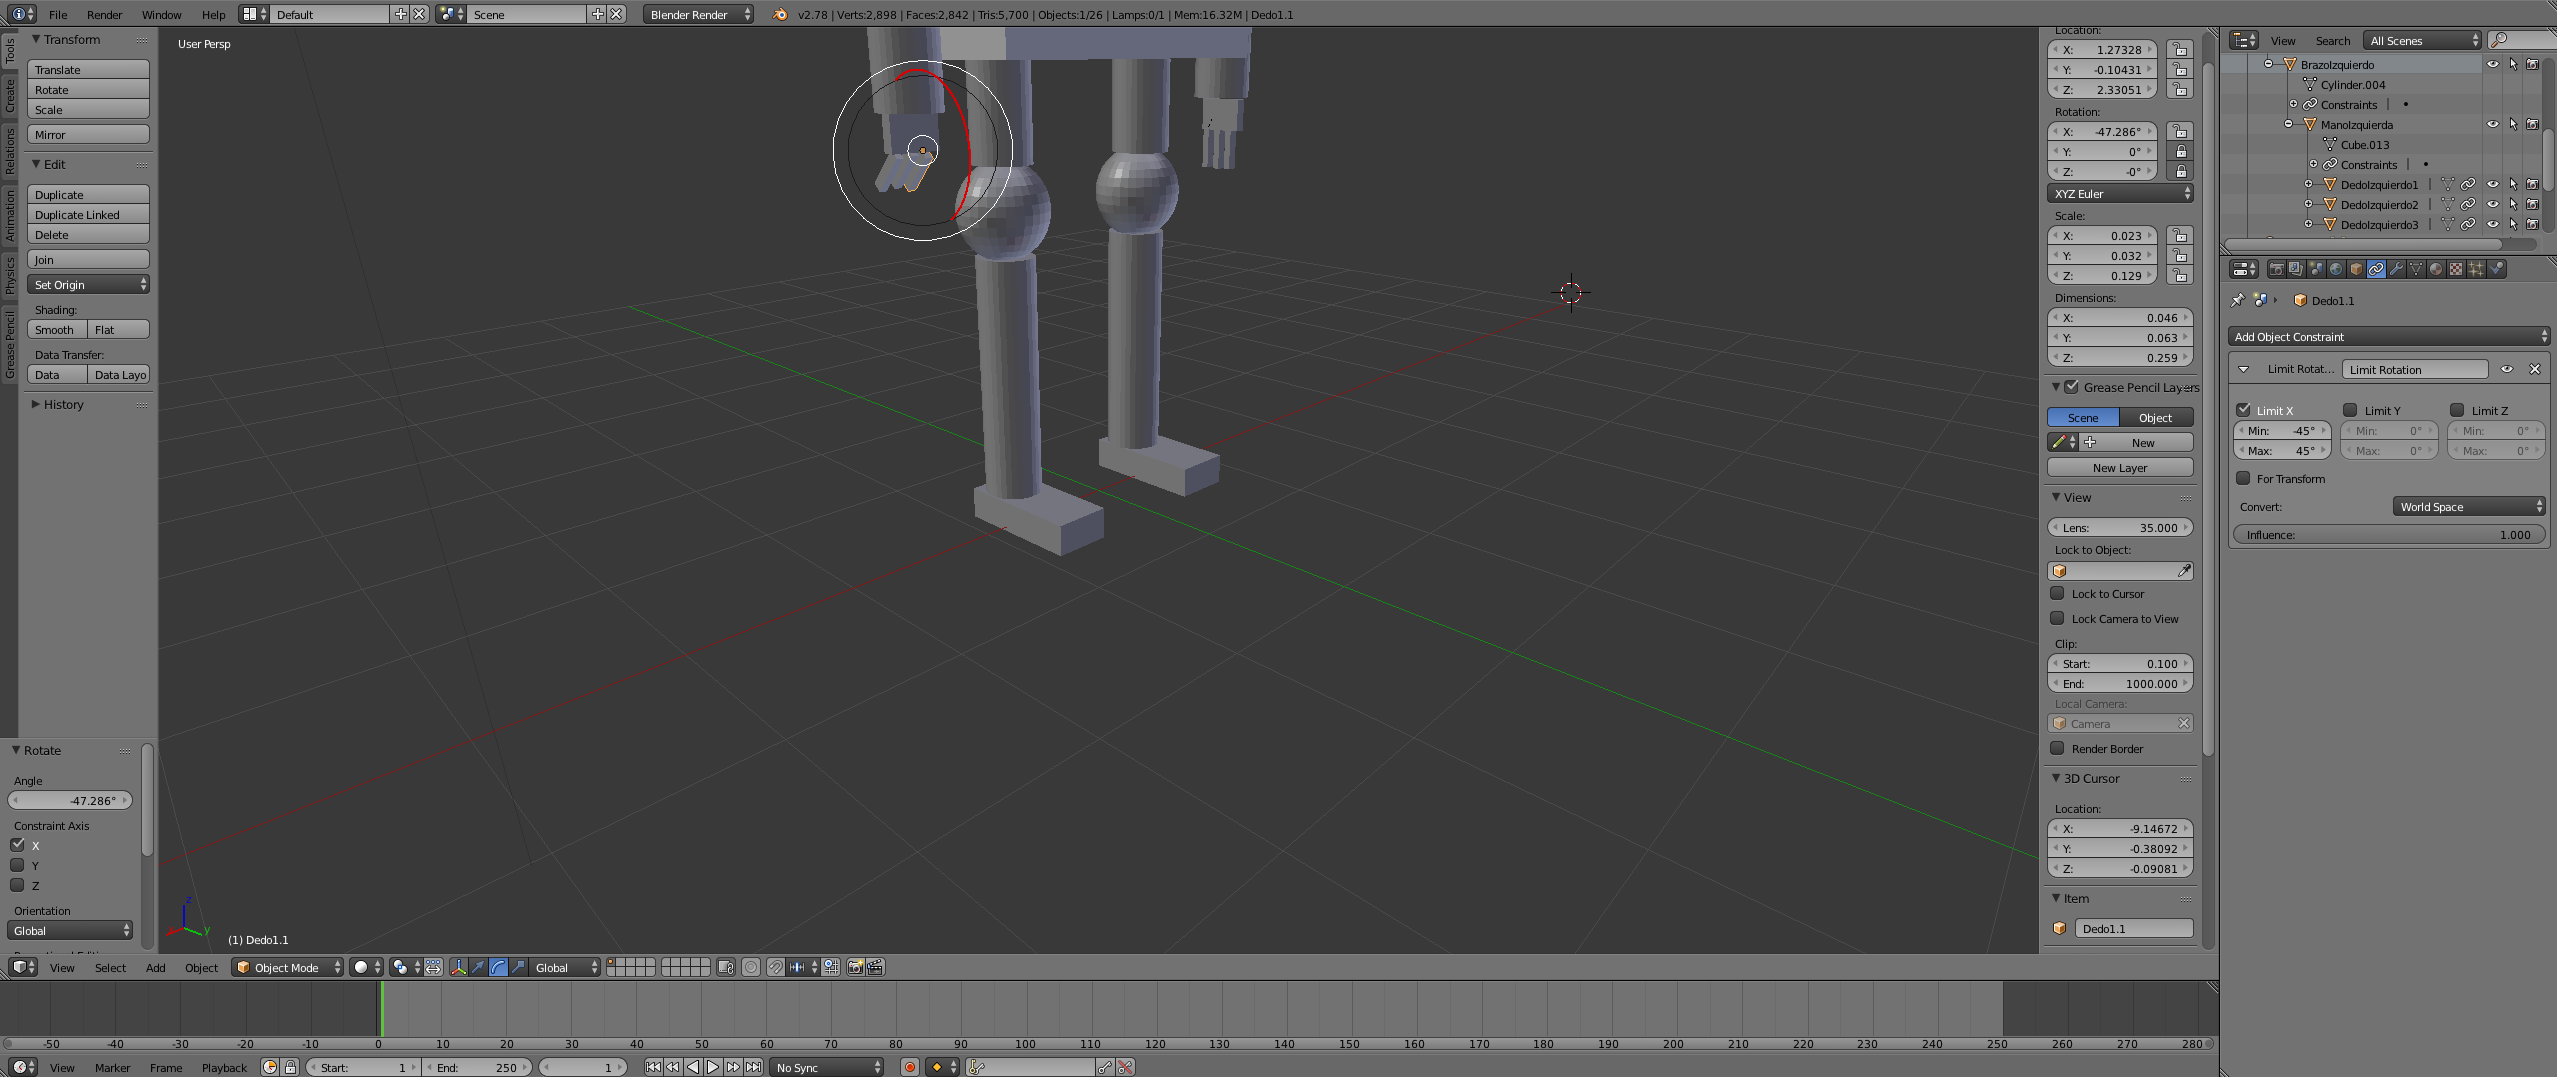
\includegraphics[width = 1.00\textwidth]{Imagenes/p2-img12.png}
 		\captionof{figure}{\label{fig:IPN}Rotación en los dedos.} 
	\end{center} 
\end{figure}

Otra de las partee de la figura ''Robot'' a la que se le han restringido las transformaciones de rotación es la representada por un cubo para el "Tronco", cuyas rotaciones en el eje X, Y y Z han sido bloqueadas conviertiéndolo en un objeto no articulado. \\

La última parte que conforma el objeto ''Robot'' es la "Pierna". Esta se compone de otro conjunto de objetos como el cuadriceps que se representa por un cilindro y que tiene restringidas las transformaciones de rotación para todos los ejes (X, Y, Z). Otro objeto que también tiene restringida las rotaciones en todos los ejes es la rodilla, que viene representada por una esfera. La pierna en sí es un objeto articulado que permite rotación limitada en el eje X con -120º como valor mínimo y 0º como máximo, siendo restringidas las rotaciones en el resto de los ejes. A este objeto que ha sido representado por un cilindro se le ha transformado el origen, poniendo este en el punto inferior de la esfera. El pie es otro de los objetos a los que se le ha modificado el punto de origen, tomando como tal el centro de la cara inferior del cilindro que representa a la pierna. El cubo que representa al pie tiene restringida la transformación de rotación en los ejes Y y Z, siendo está posible en el eje X pero limitada a -25º y 15º como valores mínimo y máximo. \\

\begin{figure}[H]
	\begin{center}
	 		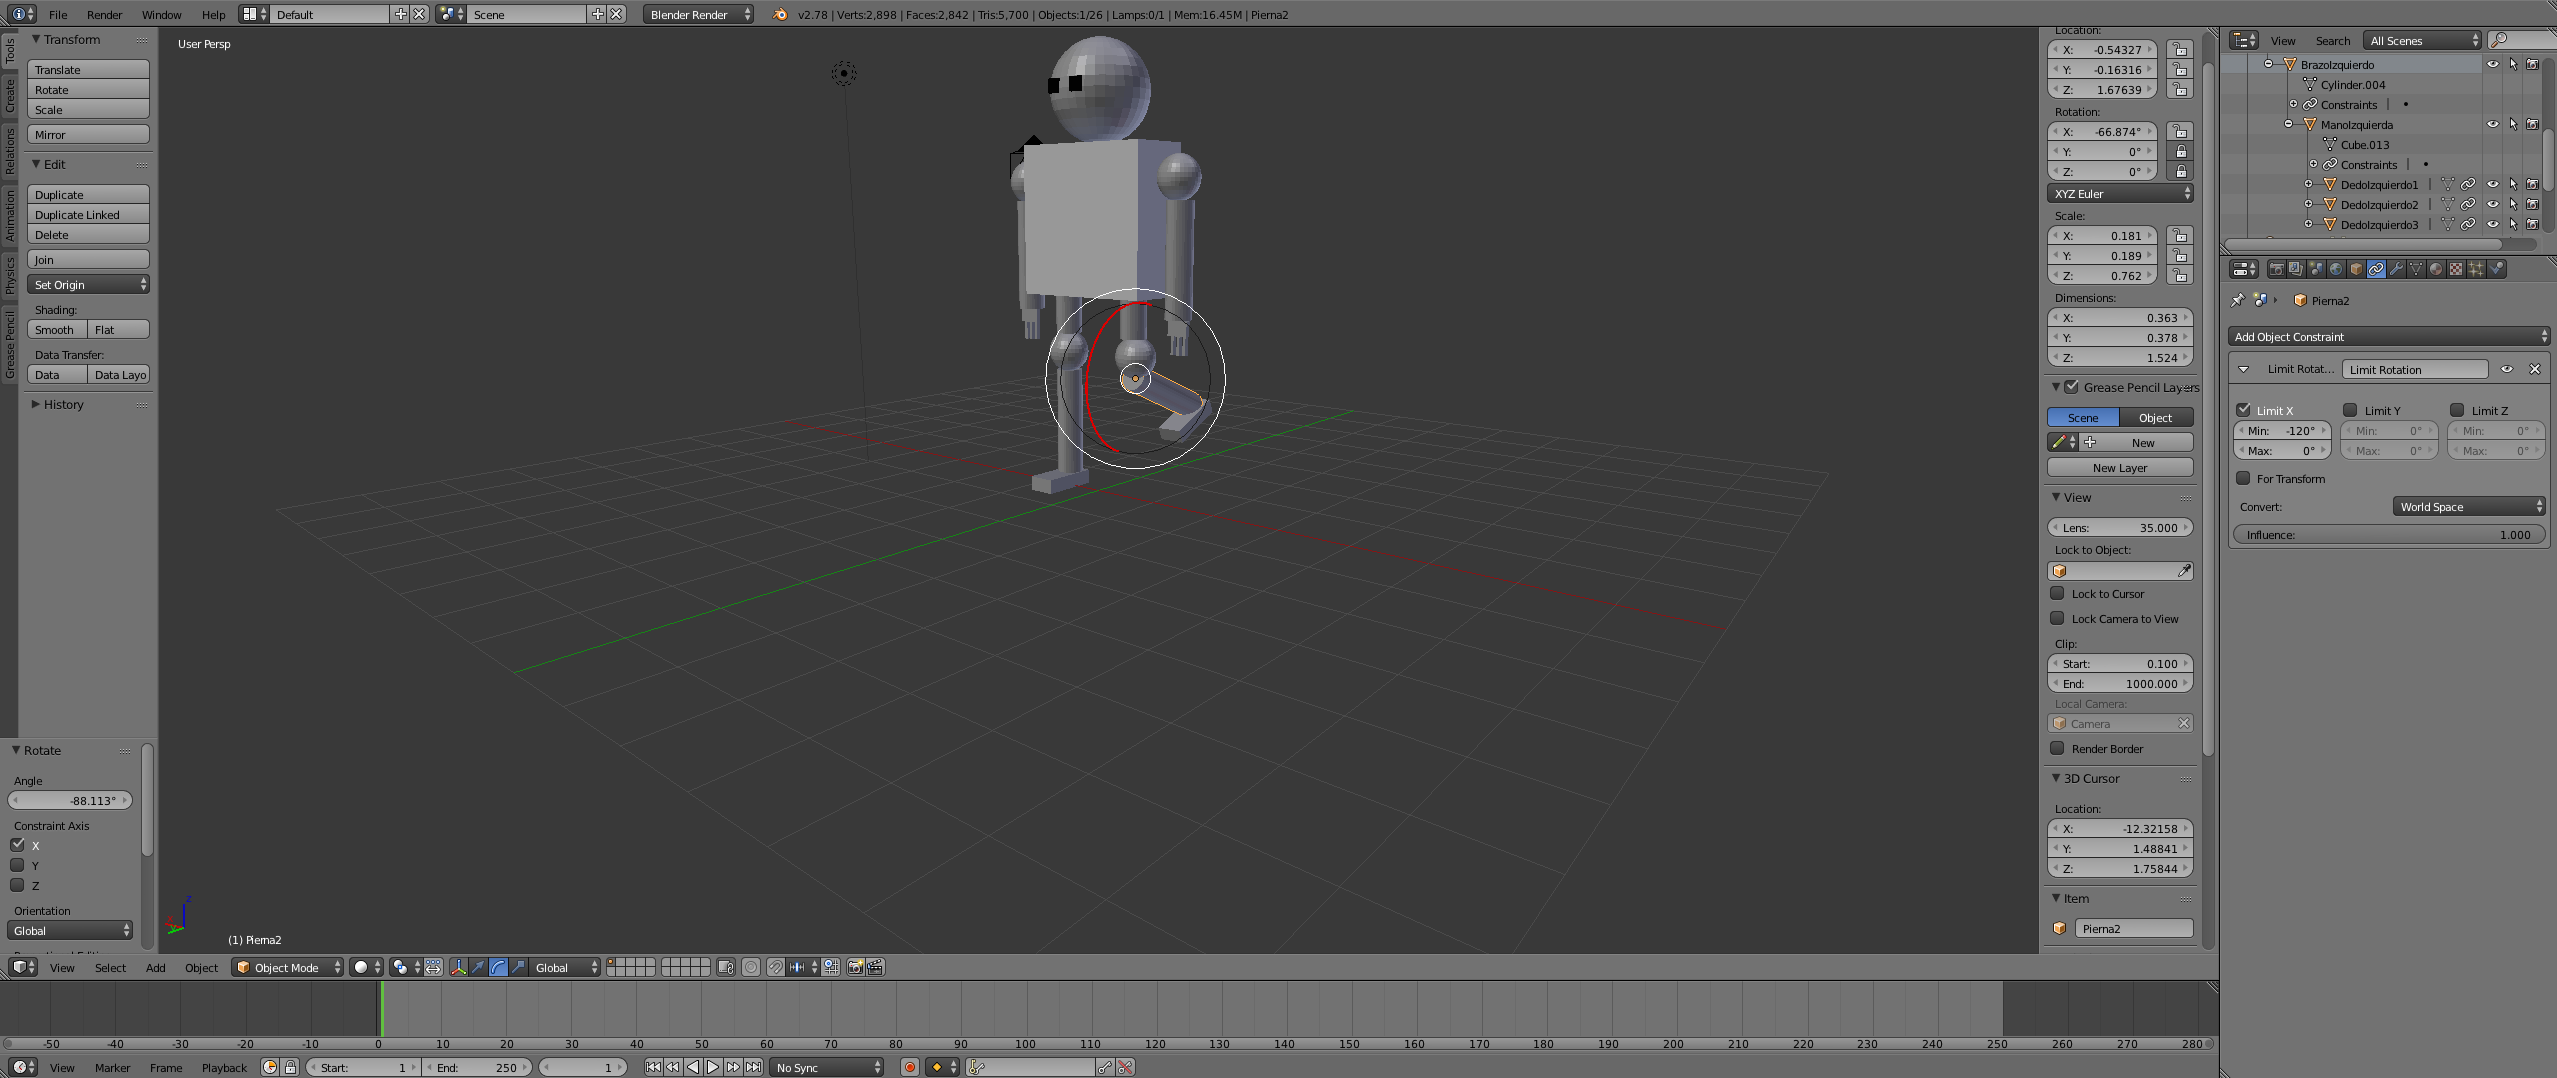
\includegraphics[width = 1.00\textwidth]{Imagenes/p2-img13.png}
 		\captionof{figure}{\label{fig:IPN}Rotación en la pierna (I).} 
	\end{center} 
\end{figure}

\begin{figure}[H]
	\begin{center}
	 		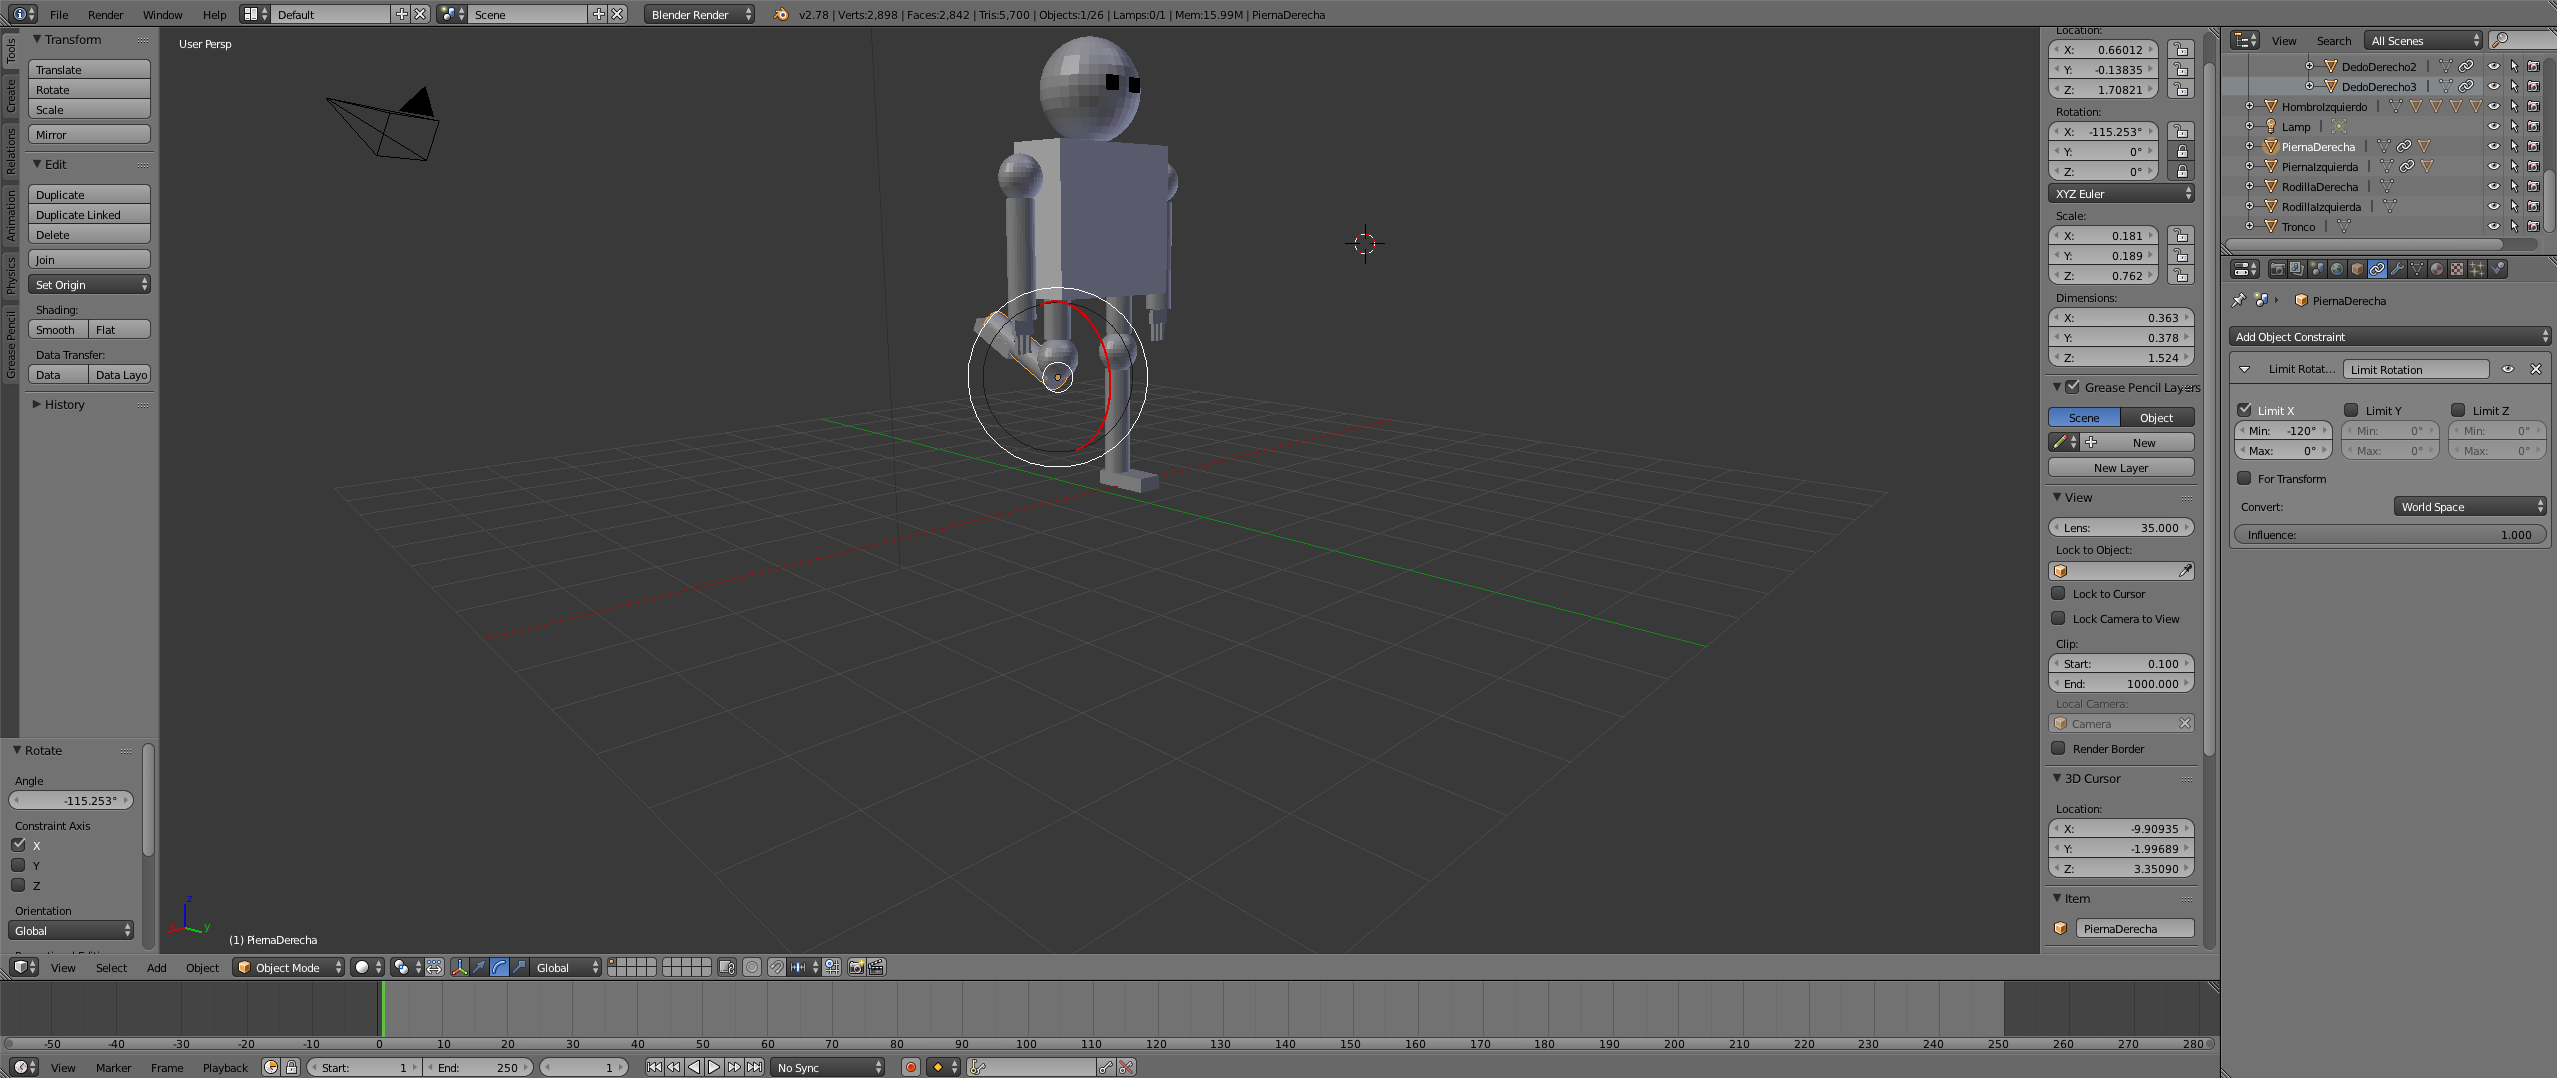
\includegraphics[width = 1.00\textwidth]{Imagenes/p2-img14.png}
 		\captionof{figure}{\label{fig:IPN}Rotación en la pierna (!I).} 
	\end{center} 
\end{figure}

\begin{figure}[H]
	\begin{center}
	 		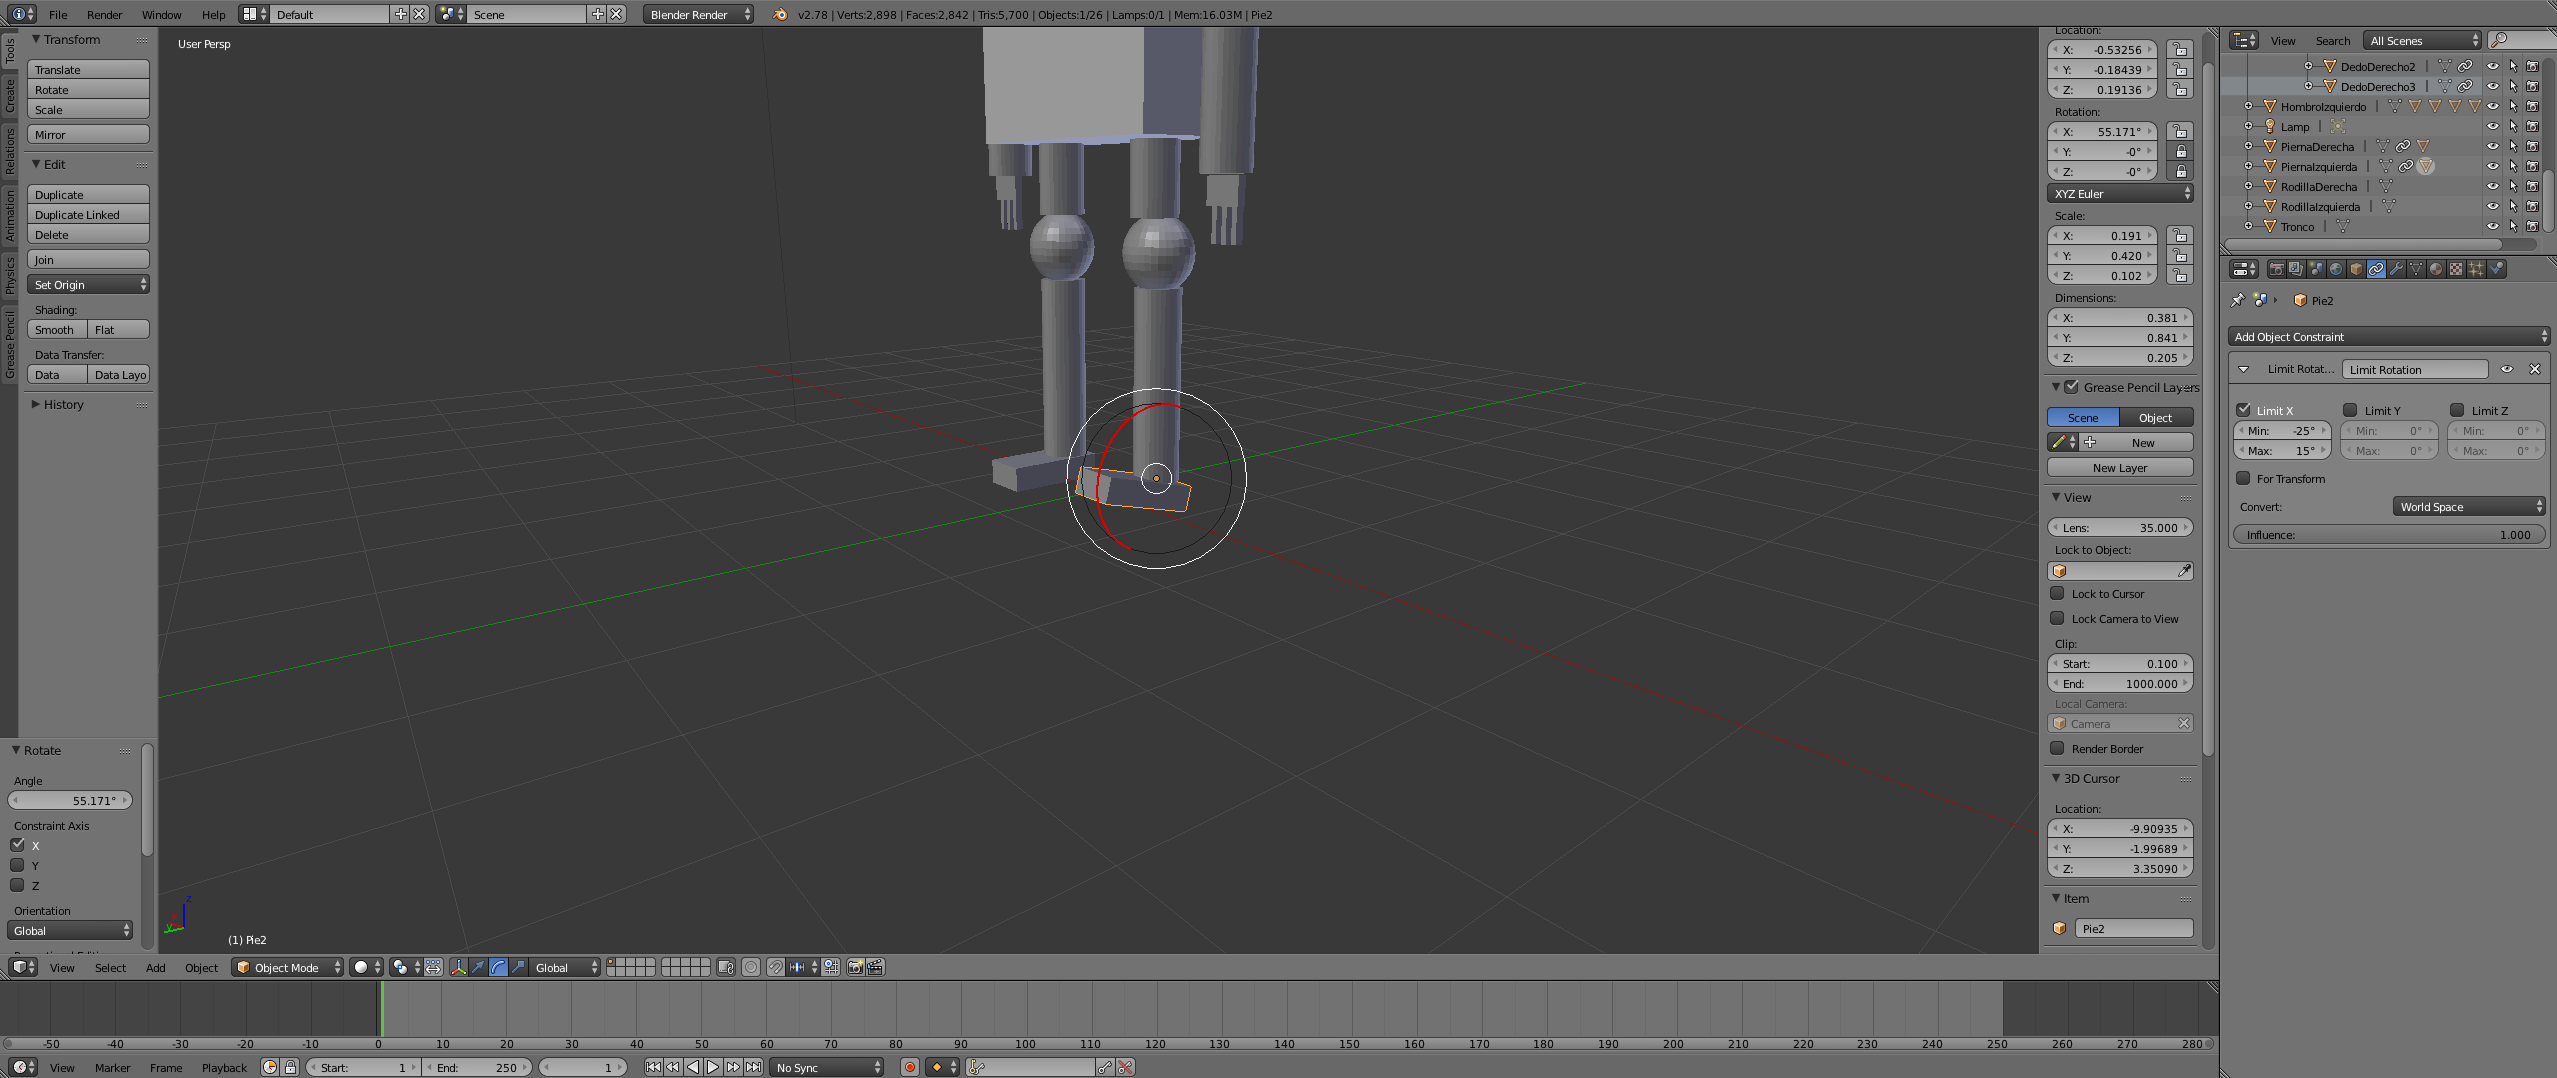
\includegraphics[width = 1.00\textwidth]{Imagenes/p2-img15.png}
 		\captionof{figure}{\label{fig:IPN}Rotación en el pie (I).} 
	\end{center} 
\end{figure}

\begin{figure}[H]
	\begin{center}
	 		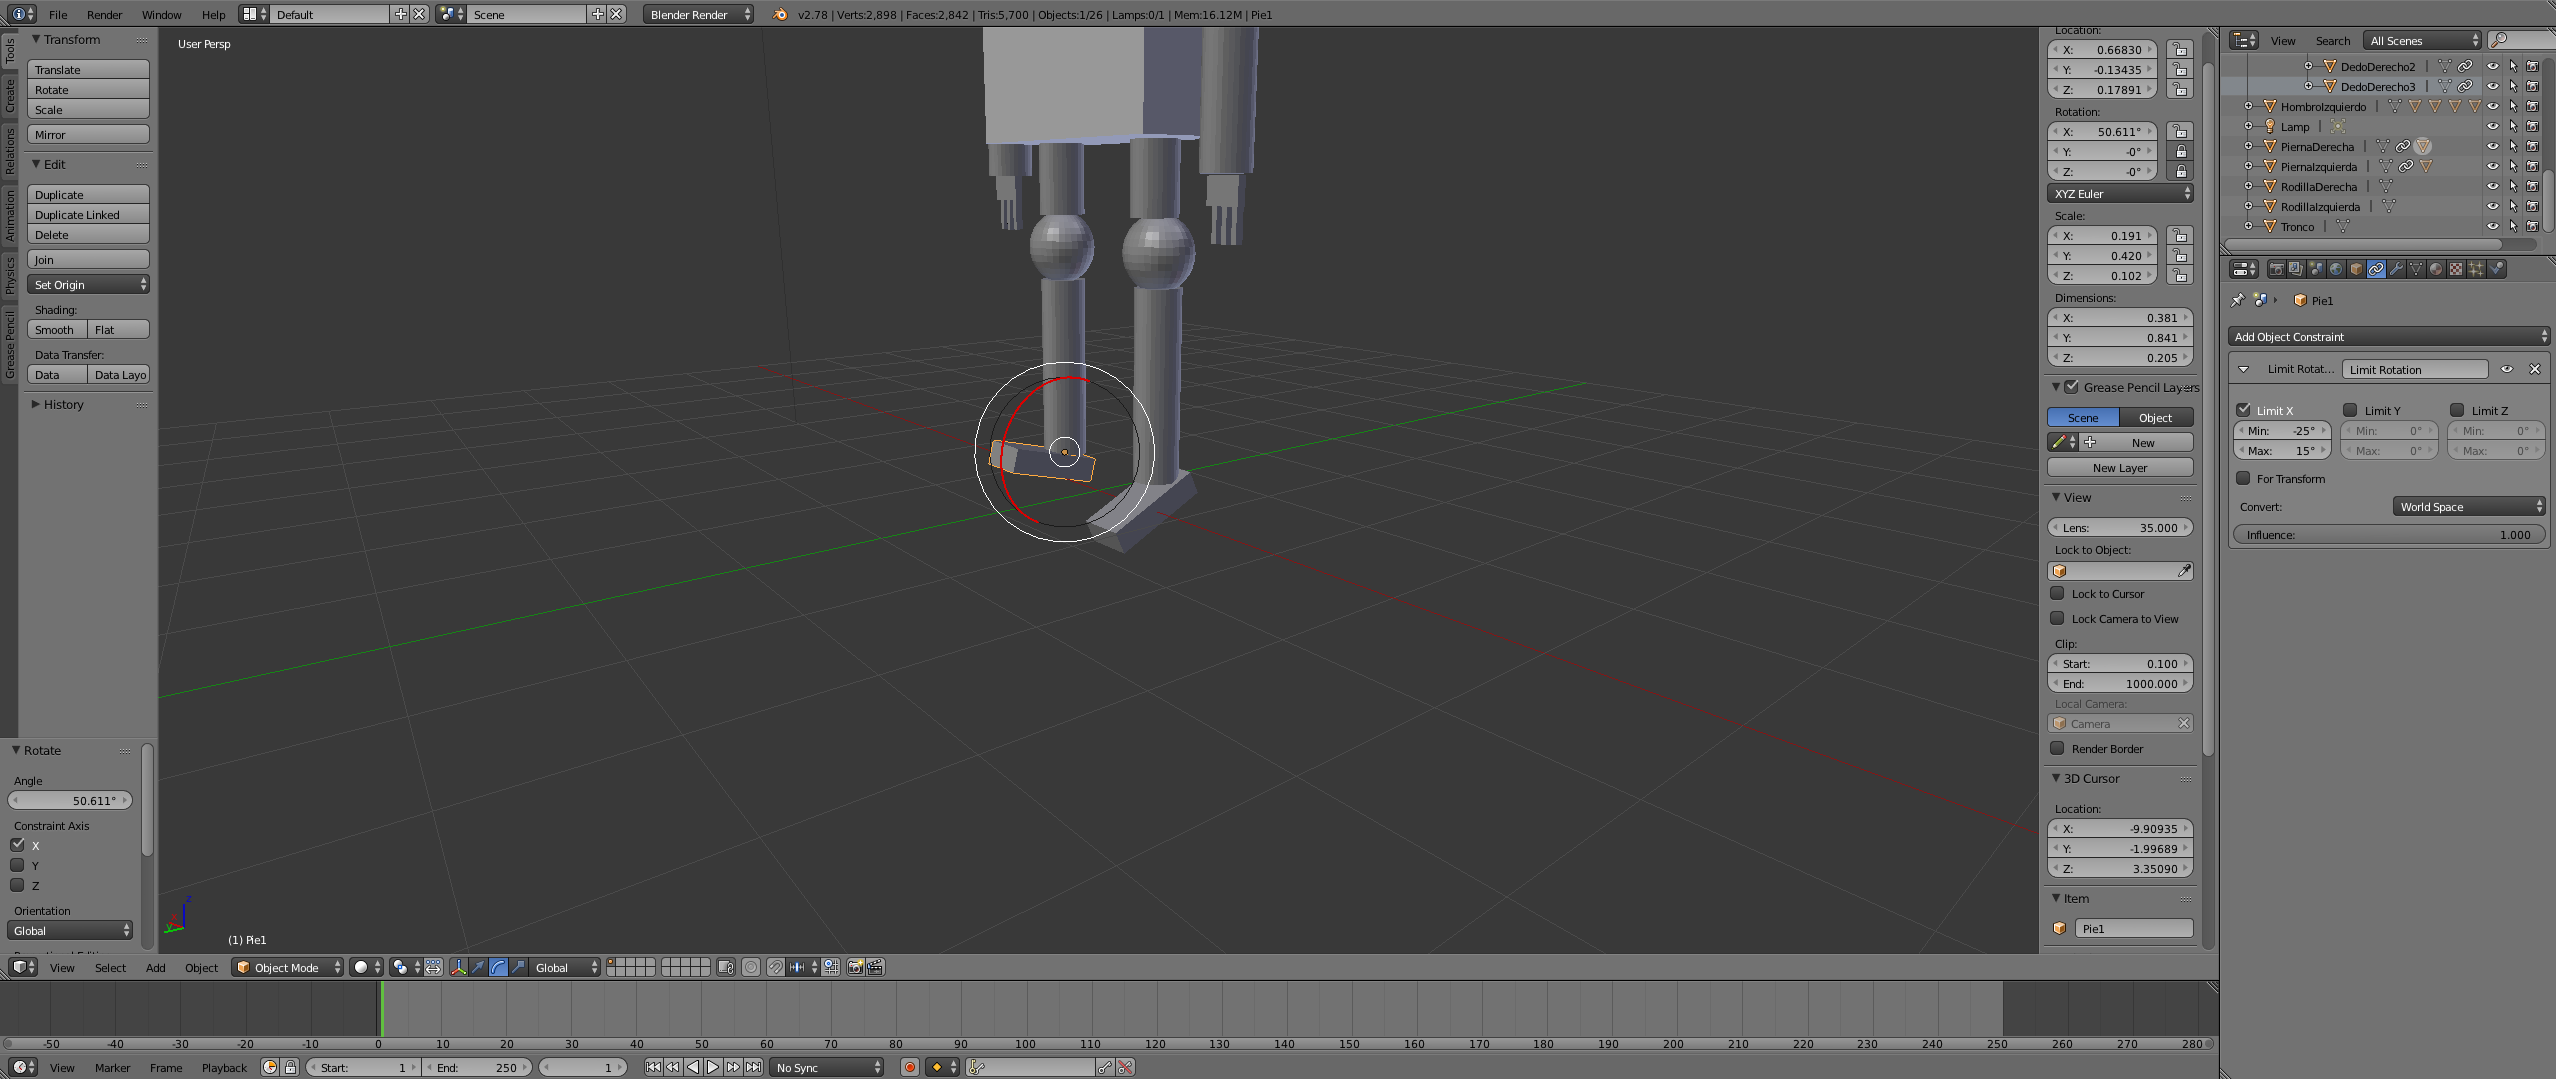
\includegraphics[width = 1.00\textwidth]{Imagenes/p2-img16.png}
 		\captionof{figure}{\label{fig:IPN}Rotación en el pie (!I).} 
	\end{center} 
\end{figure}
  

En el documento zip referente a la entrega de la práctica se encuentral fichero de blender correspondiente a la misma y la memoria donde se detallan los pasos realizados.

\end{document}